%!TEX TS-program = xelatex
%!TEX encoding = UTF-8 Unicode

\documentclass[12pt,a4paper,twoside, openright, cleardoubleempty, headsepline, footnosepline, nochapterprefix, appendixprefix, bibtotoc, abstracton]{scrreprt}

\usepackage{pdfsync}
\usepackage{ngerman}
\usepackage[ngerman]{babel}

\usepackage{multicol}
\usepackage{makeidx}
\usepackage{scrpage2}
\usepackage{natbib}

% Surround parts of graphics with box
\usepackage{boxedminipage}

% Package for including code in the document
\usepackage{listings}

% If you want to generate a toc for each chapter (use with book)
\usepackage{minitoc}

\usepackage{fontspec}
\defaultfontfeatures{Mapping=tex-text}
\setromanfont{Hoefler Text}
%\setromanfont{Gentium}
%\setromanfont{LucidaGrande}
\setsansfont{Gill Sans}
%\setsansfont{Helvetica Neue}
\setmonofont{Monaco}
\makeindex

% This is now the recommended way for checking for PDFLaTeX:
\usepackage{ifpdf}

\ifpdf
\usepackage[pdftex]{graphicx}
\else
\usepackage{graphicx}
\fi

\usepackage{geometry}

\usepackage[final, activate, verbose=true]{microtype}
\usepackage{color}

\usepackage[bookmarks]{hyperref}

\definecolor{darkgray}{gray}{0.2} 
\definecolor{lightgray}{gray}{0.8} 
\fboxrule2pt
\fboxsep10pt
\parskip1ex

\newcommand{\contribution}[1]{
	\begin{center}
	\fcolorbox{darkgray}{lightgray}{
		\begin{minipage}{13cm}
			\textbf{Kapitel \thechapter: Zusammenfassung}
			\newline
			\newline
			#1
		\end{minipage}
	}
	\end{center}
}

\newcommand{\objectives}[1]{
	\begin{center}
	\fcolorbox{darkgray}{lightgray}{
		\begin{minipage}{13cm}
			\textbf{Ziele des Kapitels \thechapter}
			\newline
			\newline
			#1
		\end{minipage}
	}
	\end{center}
}

\setcounter{tocdepth}{2}
\renewcommand*{\dictumwidth}{.5\textwidth} 
\renewcommand{\baselinestretch}{1.0}

%\usepackage[numbers]{natbib}
%\bibliographystyle{dinat}
\bibliographystyle{apalike}

\title{Diss}
\author{Stefan Oppl}
%\dedication{Für Felix und Sabrina}

\begin{document}

\pagestyle{empty}

\maketitle

%\vspace*{\fill}

\begin{center}
für \\
Felix und Sabrina
\end{center}

\vspace*{\fill}

\cleardoublepage

\section*{Vorwort} % (fold)
\label{sec:vorwort}

todo 
% section vorwort (end)

%\begin{abstract}

Der Erfolg kooperativer Arbeit beruht auf auf einem gemeinsamen Verständnis der betroffenen Abläufe durch die beteiligten Personen. Dieses gemeinsame Verständnis wird durch die ständige und unbewusste Durchführung von Articulation Work sichergestellt. In Situationen, die von den beteiligten als komplex und problematisch wahrgenommen werden, ist implizite, arbeitsbegleitende Durchführung von Articulation Work unter Umständnen nicht mehr ausreichend. Es ist dann notwendig, sich explizit mit der Abstimmung der individuellen Sichtweisen und der Bildung eines gemeinsamen Verständnisses zu beschäftigen.

Um explizite Articulation Work zu unterstützen, wird in dieser Arbeit versucht, die Interaktion der Beteiligten durch die koopertive Bildung und Diskussion diagrammatischer Modelle zu ermöglichen bzw. zu erleichtern. Dieser Zugang ist aus der Theorie der Bildung und Veränderung mentaler Modelle abgeleitet. Die Externalisierung der mentalen Modelle in Form von diagrammatischen Modellen wird dort als adäquates Mittel zur Refelexion und Kommunikation derselben identifiziert. Methodisch baut die Arbeit dabei auf Sturkturlegetechniken und Concept Mapping auf. Die dort vorgeschlagenen Methoden und Anforderungen an einer Werkzeugunterstützung werden unter Bezugnahme auf Articulation Work zusammengeführt. Die resultierende Methodik wird durch ein Tabletop Interface -- eine horizontale Interaktionsoberfläche mit rechnerbasierten Unterstützungsfunktionen -- unterstützt.

Das Werkzeug selbst wird hinsichtlich seiner Umsetzung in Hard- und Software beschrieben und einer empirischen Untersuchung unterzogen. Dabei wird die Verwendbarkeit des Werkzeugs selbst, dessen Nutzen bei der Abstimmung mentaler Modelle sowie letztendlich die Auswirkungen bei der Durchführung von Articulation Work untersucht. Die Ergebnisse deuten darauf hin, dass das Werkzeug den Anforderungen genügt und sowohl bei der Abstimmung mentaler Modelle als auch zum Teil im Kontext der durchgeführten Articulation Work zu den intendierten Wirkungen führt.
\end{abstract}

\pagestyle{scrheadings}
\automark[section]{chapter} 

\pagenumbering{roman}

\tableofcontents

\listoffigures

\listoftables

\newpage
\cleardoublepage

\pagenumbering{arabic}

%\chapter{Einführung} % (fold)
\label{cha:einführung}

\emph{„No one person embodies the requisite knowledge to comprehend complex organizational problems, or the requisite variety to clarify equivocal issues“} \citep{Tyre97}

An dieser Aussage begründen \citeauthor{Tyre97} die unbedingte Notwendigkeit zur Kooperation bei der Durchführung von Arbeit in Organisationen. Arbeit in Organisation ist ein inhärent kooperatives System \citep{Helmberger62} zur Erreichung eines Ziels \citep{Semmer04}, in dem das Ziel nur durch das Zusammenwirken der Beiträge aller beteiligten Individuen erreicht werden kann \citep{Strauss85} \citep{Tyre97}. Diese Individuen haben unterschiedliche Kenntnisse, Fähigkeiten und Interessen, die zusammengeführt und aufeinander abgestimmt werden müssen um Kooperation zu ermöglichen \citep{Schmidt94}.

\citet{Griffin92} fassen in ihrer Arbeit eine Reihe von Studien zusammen, die eine starke Korrelation zwischen funktionierender Kommunikation und Kooperation in Unternehmen und dem Erfolg neuer Produkte belegen. Auch bei Untersuchungen von Arbeitsabläufen selbst konnte die Relevanz von Kooperation zwischen Individuen bestätigt werden. Hinsichtlich der Relevanz von Kooperation zwischen Organisationen beschreiben \citet{Kumar96} die Risiken, die in organisationsübergreifenden Arbeitsprozessen auftreten können. Sowohl in klassischen organisationsübergreifenden Wertschöpfungsketten als auch in stärker vernetzten Organisationen wären den Autoren zufolge potentiellen Kosten der Kooperation zwischen den beteiligten Instanzen im Allgemeinen als das Auftretens von unterschiedlichen Interpretationen der Modalitäten der Zusammenarbeit im Speziellen wesentliche zu berücksichtigende Aspekte. \citet{Tsai02} zeigt in einer empirischen Studie die positive Wirkung von kooperationsfördernden Maßnahmen auch für Anwendungsfälle innerhalb von Organisationen. Insbesondere Tätigkeiten zur Wissensteilung und Informationsaustausch können sich demnach positiv auf Fähigkeiten der Organisation („organizational capabilities“) auswirken. \citet{Phua04} weisen die Relevanz von Kooperation auf Ebene der beteiligten Personen für Projekte im Baugewerbe empirisch nach. \citet{Roy01} zeigt anhand von Studien, dass die Abstimmung der Zusammenarbeit in Organisationen ein kritischer Erfolgsfaktor ist. Erfolgt sie nicht oder ist sie nicht erfolgreich, so leidet darunter die Fähigkeit zur Zielerreichung. Individuen, die ähnliche Denkmuster („cognitive processes“) entwickelt haben, arbeiten besser zusammen und liefern bessere Ergebnisse, als Gruppen, in denen dies nicht der Fall ist \citep{Roy01}. 

Eine Beschäftigung mit den Möglichkeiten zur Unterstützung kooperativer Arbeit und der Verbesserung derselben ist deshalb ein vielfach adressiertes Thema der Forschung vor allem in der Soziologie (etwa \citet{Strauss93} oder \citet{Suchman95}) oder den Organisationswissenschaften (etwa \citet{Argyris78}, \citet{Kim93} oder \citet{Firestone03a}) und führte auch zur Bildung neuer Forschungsfelder wie der „Computer-supported Cooperative Work“ (CSCW -- nach \citet{Grudin94} etwa ab Mitte der 1980er-Jahre). Die Einbindung von Informationtechnologie zur Unterstützung kooperativer Arbeit eröffnet neue Möglichkeiten der Zusammenarbeit und beseitigte viele Hindernisse -- vor allem jene im Zusammenhang, die im Zusammenhang mit Kommunikation und der Verfügbarkeit von Information stehen \citep{Grudin88}. Bei der Entwicklung von Systemen, die kooperative Arbeit unterstützen, müssen nach \citet{Grudin88} zwei Aspekte beachtet werden: der Verständnis der zu unterstützenden Phänomene und Abläufe in der Arbeitsrealität der betroffenen Personen\footnote{\emph{„We need to have a better understanding of how groups and organizations function and evolve than is reflected in most of the systems that have been developed. [\ldots] [One approach is to] start out with a problem situation defined by workers, and work beside them a long time in order to develop a new system that is 'owned' by the workers\ldots“} \citep[][S.90]{Grudin88}} sowie das Verständnis der Arbeitsweise der betroffenen Individuen selbst\footnote{\emph{„If we are going to support groups that include any diversity at all, we will have to learn much more about how different kinds of people work.“}\citep[][S.91]{Grudin88}}. 

Ein Ansatz, der im Rahmen von CSCW zur Erklärung kooperativer Arbeit und zur Ableitung von Unterstützungsmaßnahmen herangezogen wurde \cite{Schmidt92}, ist das Konzept der „Articulation Work“ \citet{Strauss85}. „Articulation Work“ erklärt die nach \citet{Roy01} -- wie oben zitiert -- erfolgskritischen Prozesse der Abstimmung von Zusammenarbeit und bildet die Grundlage für eine Vielzahl von Ansätzen zur Unterstützung derselben (etwa \citep{Cabitza06}, \cite{Raposo04} oder \cite{Davenport02}). In der Literatur sind jedoch keine Arbeiten zu identifizieren, die den Zusammenhang zwischen der Verwendung von „Articulation Work“ als Grundlage der Entwicklung von Unterstützungsmaßnahmen und der Berücksichtigung beider von \citet{Grudin88} formulierten Forderungen untersuchen bzw. bestätigen. Dies ist jedoch notwendig, um die Unterstützung kooperativer Arbeit in ihrer Gesamtheit -- also unter Berücksichtigung sowohl der kooperativen Arbeitsprozesse sowie der Beiträge der beteiligten Individuen -- sicherstellen zu können \citep{Grudin88}.

Das Konzept „Articulation Work“ wird von \citet{Strauss85} zur Beschreibung der unterschiedlichen Qualitäten von Tätigkeiten im Rahmen kooperativer Arbeit eingeführt. Es werden damit all jene Tätigkeiten erfasst, die der Planung und gegenseitigen Abstimmung kooperativer Arbeit sowie der Auflösung etwaig auftretender Unklarheiten oder Hindernisse bei der Zielerreichung dienen. Komplementär dazu bezeichnet \citet{Fujimura87} jenen Anteil an Arbeit, der der unmittelbaren Zielerreichung bzw. der Wertschöpfung dient, als „Production Work“. Im Sinne von Strauss dient die „Articulation Work“ also dazu, die „Production Work“ zu ermöglichen und aufrecht zu erhalten oder deren Durchführbarkeit wieder herzustellen. Entsprechend der Grundannahme von \citep{Strauss85}, dass jeder Arbeitsablauf ein inhärent kooperativer Vorgang ist, ermöglicht bzw. erhält „Articulation Work“ also eine funktionierende Kommunikation und Zusammenarbeit in Arbeitsabläufen. Zentral ist dabei vor allem die gegenseitigen Offenlegung der Annahmen aller beteiligten Personen, die den individuellen Arbeitsbeiträgen zugrunde liegen\footnote{\emph{„Reconciling incommensurate assumptions and procedures in the absence of enforceable standards is the essence of articulation.“}\citep[][S. 266]{Gerson86}}. Die Arbeiten von Strauss haben rein deskriptiven Charakter, sie beschreiben das beobachtbare Phänomen des Auftretens von „Articulation Work“, treffen aber keine Aussagen über deren Wirkmechanismen oder etwaige Möglichkeiten zur Unterstützung derselben.

„Articulation Work“ ist nach Strauss integraler Bestandteil jedes kooperativen Arbeitsablaufs. Jene sozialen, unbewusst ausgeführten Tätigkeiten, die der Abstimmung der individuellen Arbeitsbeiträge dienen, bezeichnet \citet{Strauss88} bzw. \citet{Fjuk97} als \emph{implizite} „Articulation Work“.  Mit steigender Komplexität der „Production Work“ steigt auch der Aufwand der dazu notwendigen „Articulation Work“ an \citep{Strauss88}. Die Komplexität steigt hier mit der Anzahl der benötigten Arbeitsschritte, den dazu benötigten Kompetenzen und der Anzahl der involvierten Personen. Je komplexer („problematic“) eine Interaktion ist, desto notwendiger wird nach \citep{Strauss88} eine explizite Beschäftigung mit dem Vorgang der Artikulation. Werden Tätigkeiten in diesem Rahmen bewusst durchgeführt, so spricht man von \emph{expliziter} „Articulation Work“ \citep{Strauss88} \citep{Fjuk97}. 

Der Begriff der „problematischen Interaktion“ bedarf einer näheren Betrachtung, um als Kriterium der Abgrenzung zwischen impliziter und expliziter „Articulation Work“ herangezogen werden zu können. Strauss zitiert diesbezüglich Hughes unmittelbar nach seiner Definition von „problematic interaction“: \emph{„[O]ne man's routine of work is made up of the emergencies of other people“} \citep[][zitiert nach \citep{Strauss93}]{Hughes71}. Das Merkmal, an dem die Notwendigkeit der Durchführung expliziter „Articulation Work“ begründet wird, ist demnach also ausschließlich durch individuelle Wahrnehmung beurteilbar. Die bewusste Durchführung von Abstimmungsaktivitäten ist immer dann notwendig, wenn zumindest eine der beteiligten Personen die Arbeitssituation als „problematisch“ wahrnimmt. Wie bereits oben erwähnt, beschreibt Strauss in seinen Arbeiten zwar das Phänomen „Articulation Work“ und dessen Wirkung (also im Wesentlichen \emph{was} „Articulation Work“ ist), verzichtet aber auf eine detaillierte Betrachtung der Abläufe und Tätigkeiten bei der Durchführung der derselben (also \emph{wie} „Articulation Work“ funktioniert). Insbesondere ignoriert er den individuellen Aspekt von „Articulation Work“, also jene die kognitiven Phänomene, die durch „Articulation Work“ beeinflusst werden bzw. die die Auslöser für deren Durchführung sind. Strauss ist sich dieser Auslassung bewusst\footnote{\emph{„[\ldots] many social scientist pay almost no attention to interior activity: ignoring it, taking it for granted, but leaving it unexamined, or giving it the kind of abstract but not very detailed analysis [\ldots]“}\citep[][S. 131]{Strauss93}}, und bezeichnet diese kognitiven Vorgänge in späteren Arbeiten (etwa \citep{Strauss93})  als wichtig für das Verständnis der Abläufe bei der Durchführung von „Articulation Work“, ohne jedoch näher auf diese einzugehen. Diese Auslassung führt dazu, dass die von \citet{Grudin88} formulierte Forderung nach einem Verständnis der individuellen Arbeitsweisen bei kooperativer Arbeit bei der ausschließlichen Verwendung des Konzepts der „Articulation Work“ nicht erfüllt werden kann. Dies hat Auswirkungen auf spätere Arbeiten anderer Autoren, die sich der Unterstützung von „Articulation Work“ widmen (etwa \citet{Schmidt92}, \citet{Simone99} oder \citet{Baker07}).

Durch die Fokussierung auf die soziale Dimension von Arbeit im Allgemeinen und „Articulation Work“ im Besonderen berücksichtigen die vorgeschlagenen Unterstützungsansätze ebenfalls vorrangig auf die Unterstützung sozialen (Kommunikations-)Prozesse. Als Konsequenz sind die meisten Ansätze vor allem zur Unterstützung impliziter „Articulation Work“ geeignet und berücksichtigen die Möglichkeit des Auftretens „problematischer Interaktionen“ nicht explizit. Deutlich wird dies beispielsweise bei den Arbeiten von \citep{Sarini02} -- die Autoren schlagen ein System vor, dass die Durchführung von „Articulation Work“ in domänenübergreifenden Arbeitssituationen unterstützen soll -- ein wesentliches Problem ist den Autoren zufolge hier die Sicherstellung eines gemeinsamen Begriffsverständnisses. Der Ansatz der Unterstützung im Arbeitsablauf selbst wird detailliert beschrieben. Durch die rechnerbasierte Identifikation und Anzeige analoger Begrifflichkeiten aus den betroffenen Domänen soll der soziale Kommunikationsprozess ermöglicht bzw. erleichtert werden. Der Aspekt der Erhebung der Begrifflichkeiten und deren Zuordnung zueinander -- also jener Aspekt, der die einzelnen Individuen und deren Wahrnehmung der Domänen involviert -- wird nur am Rande und eher oberflächlich behandelt\footnote{\emph{„For sake of testing the integration we are aiming at, we defined the simplest protocol: all the users involved in the reconciliation process can communicate among themselves to define the correspondences, while a single Actor assumes the Role of Manager of the Reconciliation Artifact and is in charge of keeping it updated.“}\citep[][S. 10]{Sarini02}}. 

Arbeiten, die sich mit dem Vorgang der Abstimmung von Arbeit beschäftigen, ohne sich explizit auf Strauss' Konzept von „Articulation Work“ zu beziehen (wie etwa \citep{Jorgensen04}), berücksichtigten häufig auch stärker den Aspekt der konkreten Durchführung von „Articulation Work“ und eignen sich durch ihren Fokus auf die dezidierte Unterstützung des Abstimmungsprozesses an sich (und nicht nur die Schaffung der dazu notwendigen Rahmenbedingungen) auch für explizite „Articulation Work“. Auch in diesen Fällen erfolgt jedoch die Berücksichtigung der Rolle der beteiligten Individuen und deren Unterstützung nur in Einzelfällen (etwa bei \citet{Herrmann02}), womit die Forderung von \citet{Grudin88} wiederum nicht erfüllt werden können.

Die Unterstützung expliziter „Articulation Work“ ist also ein bislang nur selten explizit adressiertes Themenfeld. Durch die historische Entwicklung des Forschungsgebiets bedingt wurde die Rolle der beteiligten Individuen dabei nur am Rande berücksichtigt (was wiederum zur Fokussierung auf Maßnahmen zu führt, die auf die Unterstützung von sozialen Abstimmungsprozessen im Arbeitsablauf -- also impliziter „Articulation Work“ -- abzielen). In dieser Arbeit werden deshalb die Möglichkeiten zur Unterstützung expliziter „Articulation Work“ durch die Berücksichtigung der Rolle der beteiligten Individuen erfasst und daraus ein konkretes Unterstützungsinstrument entwickelt. Um die tatsächliche Unterstützung von „Articulation Work“ nachzuweisen, wird dessen Effektivität im Kontext der „Production Work“ geprüft. Zusammengefasst kann die globale Zielsetzung dieser Arbeit wie folgt beschreiben werden:

\begin{framed}
	\label{zielsetzung}\textbf{Globale Zielsetzung} 
	
	\emph{In der vorliegenden Arbeit sind die Möglichkeiten zur methodischen Unterstützung von expliziter Articulation Work unter Berücksichtigung relevanter Theoriebildungen zur Rolle der beteiligten Individuen zu erfassen, auf Basis dieser Erkenntnisse geeignete Methoden auszuwählen, diese in einem Instrument umzusetzen und dessen Effektivität im Kontext der Production Work zu prüfen.}
\end{framed}


\section{Forschungsfragen} % (fold)
\label{sec:forschungsfragen}

Aus der oben formulierten globalen Zielsetzung müssen zur strukturierten Bearbeitung detaillierte Fragestellungen abgeleitet werden. Die formulierten Forschungsfragen und deren detaillierte Fragestellungen bilden die Ankerpunkte des inhaltlichen Aufbaus dieser Arbeit und werden in allen folgenden Kapiteln referenziert, um den Bezug zur globalen Zielsetzung herzustellen. In Abbildung \ref{fig:img_Einfuehrung_zielhierarchie} sind die Forschungsfragen und Fragestellungen sowie deren Beziehung untereinander nochmals graphisch dargestellt.

In der globalen Zielsetzung wird die Unterstützung expliziter „Articulation Work“ gefordert. Um diese Forderung zu erfüllen, ist es notwendig, das Konzept der „Articulation Work“ zu untersuchen, um Ansatzpunkte für die exakte Abgrenzung expliziter „Articulation Work“, deren Unterstützung sowie der Beurteilung der effektiven Durchführung derselben zu erfassen. Dies ist Gegenstand der ersten Forschungsfrage. 

\begin{ff}
	\label{ff:beschreibung}
	Wie kann die Durchführung und Wirkung von „Articulation Work“ charakterisiert werden?
\end{ff}

Im Rahmen der ersten Forschungsfrage können mehrere voneinander unabhängig zu bearbeitende Fragestellungen identifiziert werden, deren Beantwortung und Verknüpfung letztendlich zur Beantwortung der Forschungsfrage selbst führt.

Ein Aspekt der ersten Forschungsfrage ist die Klärung des Begriffs „Articulation Work“ selbst. Oben wurde bereits angedeutet, wie „Articulation Work“ von anderen Teilen eines Arbeitsablaufs abgegrenzt werden kann. Die Beschreibung der Durchführung von „Articulation Work“, also der möglichen Tätigkeiten und Rahmenbedingungen, bedarf aber einer detaillierten Betrachtung der existierenden Literatur. Die Wirkung von „Articulation Work“ (also: „Woran zeigen sich Konsequenzen der Durchführung von Articulation Work und wie können diese ausgeprägt sein?“) muss ebenfalls Gegenstand der Betrachtung sein, um Ansatzpunkte zur Beurteilung deren Effektivität identifizieren zu können. Aus diesen beiden Aspekten ergibt sich Fragestellung \ref{tf:was_is_aw}.

\begin{tf}
	\label{tf:was_is_aw}
	Was ist „Articulation Work“ und wie wirkt sie im Arbeitsprozess?
\end{tf}

„Articulation Work“ dient der Beseitigung „problematischer“ Situationen in der „Production Work“. Die Einschätzung, ob eine Situation „problematisch“ ist und ob die „Probleme“ beseitigt wurden, obliegt jedoch der subjektiven Einschätzung der handelnden Individuen. Auch die Entscheidung zur Durchführung expliziter „Articulation Work“ (aufgrund von implizit nicht auflösbaren wahrgenommenen „Problemen“) obliegt den involvierten Personen. Die Durchführung von „Articulation Work“ ist damit wesentlich von den handelnden Individuen beeinflusst, wird von diesen angestossen und auch wieder beendet. Für die Betrachtung der Möglichkeiten zur Unterstützung von „Articulation Work“ ist es deshalb von Interesse, wie die beteiligten Individuen beurteilen, ob eine Situation „problematisch“ ist und ob dies nach der Durchführung von Tätigkeiten im Rahmen von „Articulation Work“ nicht mehr der Fall ist (und diese deshalb beendet werden kann). Der Aspekt der individuellen Wahrnehmung und Denkprozesse wird von \citet[][S. 131]{Strauss93} als wichtig für die Erklärung von „Articulation Work“ bezeichnet, jedoch explizit nicht weiter betrachtet. Zur Beantwortung der Fragestellung \ref{tf:rolle_der_individuen} ist deshalb die Betrachtung anderer, auf die Wahrnehmungs- und Denkprozesse der beteiligten Individuen eingehender Theorien notwendig.

\begin{tf}
	\label{tf:rolle_der_individuen}
	Wie kann die Wahrnehmung von Arbeitsabläufen durch die an diesen beteiligten Individuen erklärt werden?
\end{tf}

Die Beantwortung der beiden bisher formulierten Fragestellungen ermöglicht eine umfassende Charakterisierung von „Articulation Work“ sowohl hinsichtlich deren Durchführung als auch deren Wirkung auf die „Production Work“. Die Beantwortung der Forschungsfrage geht insofern über den aktuellen Stand der Literatur hinaus, als dass sie auch die beteiligten Individuen vor, während und nach der Durchführung von „Articulation Work“ in die Betrachtung mit einbezieht. Durch die Erweiterung des Betrachtungsbereichs ergeben sich potentiell neue Ansatzpunkte für die Unterstützung von „Articulation Work“, die in der zweiten Forschungsfrage erfasst werden sollen.

\begin{ff}
	\label{ff:umsetzung}
	Wie kann explizite „Articulation Work“ effektiv unterstützt werden?
\end{ff}

Auch die zweite Forschungsfrage bedarf zur umfassenden Bearbeitung der Unterteilung in mehrere Fragestellungen, die sich aus der Formulierung der globalen Zielsetzung ergeben. Im Gegensatz zur ersten Forschungsfrage sind die Fragestellung hier nicht unabhängig voneinander bearbeitbar sondern bauen zum Teil aufeinander auf. Die ersten beiden Fragestellungen beschäftigen sich mit der Unterstützung von „Articulation Work“ und stellen sowohl die methodischen Möglichkeiten als auch die konkrete Umsetzung dar. Die zweiten beiden Fragestellungen fokussieren auf die geforderte „effektive Unterstützung“. Hier wird im ersten Schritt geklärt, woran sich die effektive Unterstützung von „Articulation Work“ zeigt und wie diese beurteilt werden kann. Im zweiten Schritt wird das umgesetzte Instrument in diesem Sinne geprüft. 

Bei der Betrachtung der Unterstützungsmöglichkeiten für „Articulation Work“ muss zwischen deren impliziter und expliziter Ausprägung unterschieden werden. Implizite „Articulation Work“ ist ein nicht formalisierter Prozess, der von den beteiligten Individuen unbewusst durchgeführt wird. Die Unterstützungsmöglichkeiten beschränken sich hier auf die Schaffung der sozialen bzw. technologischen Rahmenbedingungen, die die Durchführung impliziter „Articulation Work“ ermöglichen. Explizite „Articulation Work“ basiert hingegen auf der bewussten Beschäftigung der Individuen mit der „problematischen“ Arbeit. Sie hat das Ziel, einen Zustand herzustellen, in dem implizite „Articulation Work“ (wieder) möglich ist, d.h. in dem die beteiligten Individuen die Situation nicht mehr als zu komplex bzw. „problematisch“ wahrnehmen. Bei der Unterstützung expliziter „Articulation Work“ ist es deshalb sinnvoll, vor allem auch Methoden zur Unterstützung der Individuen im Prozess der Durchführung von „Articulation Work“ zu erfassen.

\begin{tf}
	\label{tf:methoden}
	Welche Methoden können zur Unterstützung von „Articulation Work“ herangezogen werden?
\end{tf}

Wie oben bereits erwähnt, ist die Unterstützung impliziter „Articulation Work“ ein umfassend erforschtes Gebiet, während kaum Arbeiten zur Unterstützung expliziter „Articulation Work“ vorhanden sind. Diese Hypothesen werden durch die Beantwortung der Fragestellung \ref{tf:methoden} verifiziert. Gelingt dies, kann an dieser Stelle auf die Unterstützung expliziter „Articulation Work“ fokussiert werden. Die ermöglicht gleichzeitig eine Fokussierung auf Methoden, die im Sinne der obigen Ausführungen die beteiligten Individuen bei der Durchführung von expliziter „Articulation Work“ unterstützen. Diese Methoden sind in der Folge in einem Instrument umzusetzen. Als „Instrument“ wird an dieser Stelle die Gesamtheit aller Maßnahmen zur Unterstützung der Durchführung der Methoden bezeichnet. Die Auswahl der geeigneten Methoden sowie die Umsetzung in einem Instrument sind Gegenstand der Fragestellung \ref{tf:technik}.

\begin{tf}
	\label{tf:technik}
	Wie kann ein Instrument zur Unterstützung von expliziter „Articulation Work“ umgesetzt werden?
\end{tf}

Die Forderung nach einer effektiven Unterstützung von expliziter „Articulation Work“ bedingt die Festlegung des Effektivitätskriteriums. Unter Berücksichtigung der obigen Ausführungen sind einerseits die Durchführung (sowohl deren grundsätzliche Ermöglichung als auch die Durchführung im Sinne der vorgeschlagenen Methodik) und andererseits die Wirkung der „Articulation Work“ (sowohl auf individueller Ebene als auch auf Ebene der „Production Work“) mögliche Merkmale, die hinsichtlich der Effektivität der Unterstützung beobachtet werden können. Die Festlegung der konkreten Form der Beurteilung hängt von den Ergebnissen der Forschungsfrage 1 ab und wird im Rahmen der Bearbeitung von Fragestellung \ref{tf:beurteilung_der_effektivität} beantwortet.

\begin{tf}
	\label{tf:beurteilung_der_effektivität}
	Wie kann die Effektivität der Unterstützung von expliziter „Articulation Work“ beurteilt werden?
\end{tf}

Die Beurteilung des umgesetzten Instruments anhand des Kriteriums der effektiven Unterstützung von „Articulation Work“ bildet den letzten Schritt in der Bearbeitung der Forschungsfrage \ref{ff:umsetzung}. Die Beantwortung der Forschungsfrage ist nur dann möglich, wenn das aus der Theorie abgeleitete Instrument tatsächlich eine Möglichkeit zur effektiven Unterstützung von „Articulation Work“ darstellt. Zur Bearbeitung dieser Fragestellung müssen sowohl die Fragestellung \ref{tf:technik} als auch die Fragestellung \ref{tf:beurteilung_der_effektivität} abgeschlossen sein.

\begin{tf}
	\label{tf:empirie}
	Ermöglicht das Instrument die effektive Durchführung von expliziter „Articulation Work“?
\end{tf}

Die Beantwortung der Forschungsfrage \ref{ff:umsetzung} erfolgt durch die Darstellung eines möglichen Instruments für die Unterstützung expliziter „Articulation Work“. Kann die Effektivität der Unterstützung durch dieses Instruments bestätigt werden, so kann bei Beantwortung aller vorangegangener Fragestellungen auch die globale Zielsetzung als erfüllt angesehen werden.

Die Zusammenhänge zwischen der globalen Zielsetzung, den Forschungsfragen und den einzelnen Fragestellungen sind in Abbildung \ref{fig:img_Einfuehrung_zielhierarchie} nochmals graphisch zusammengefasst. 

\begin{figure}[htbp]
	\centering
		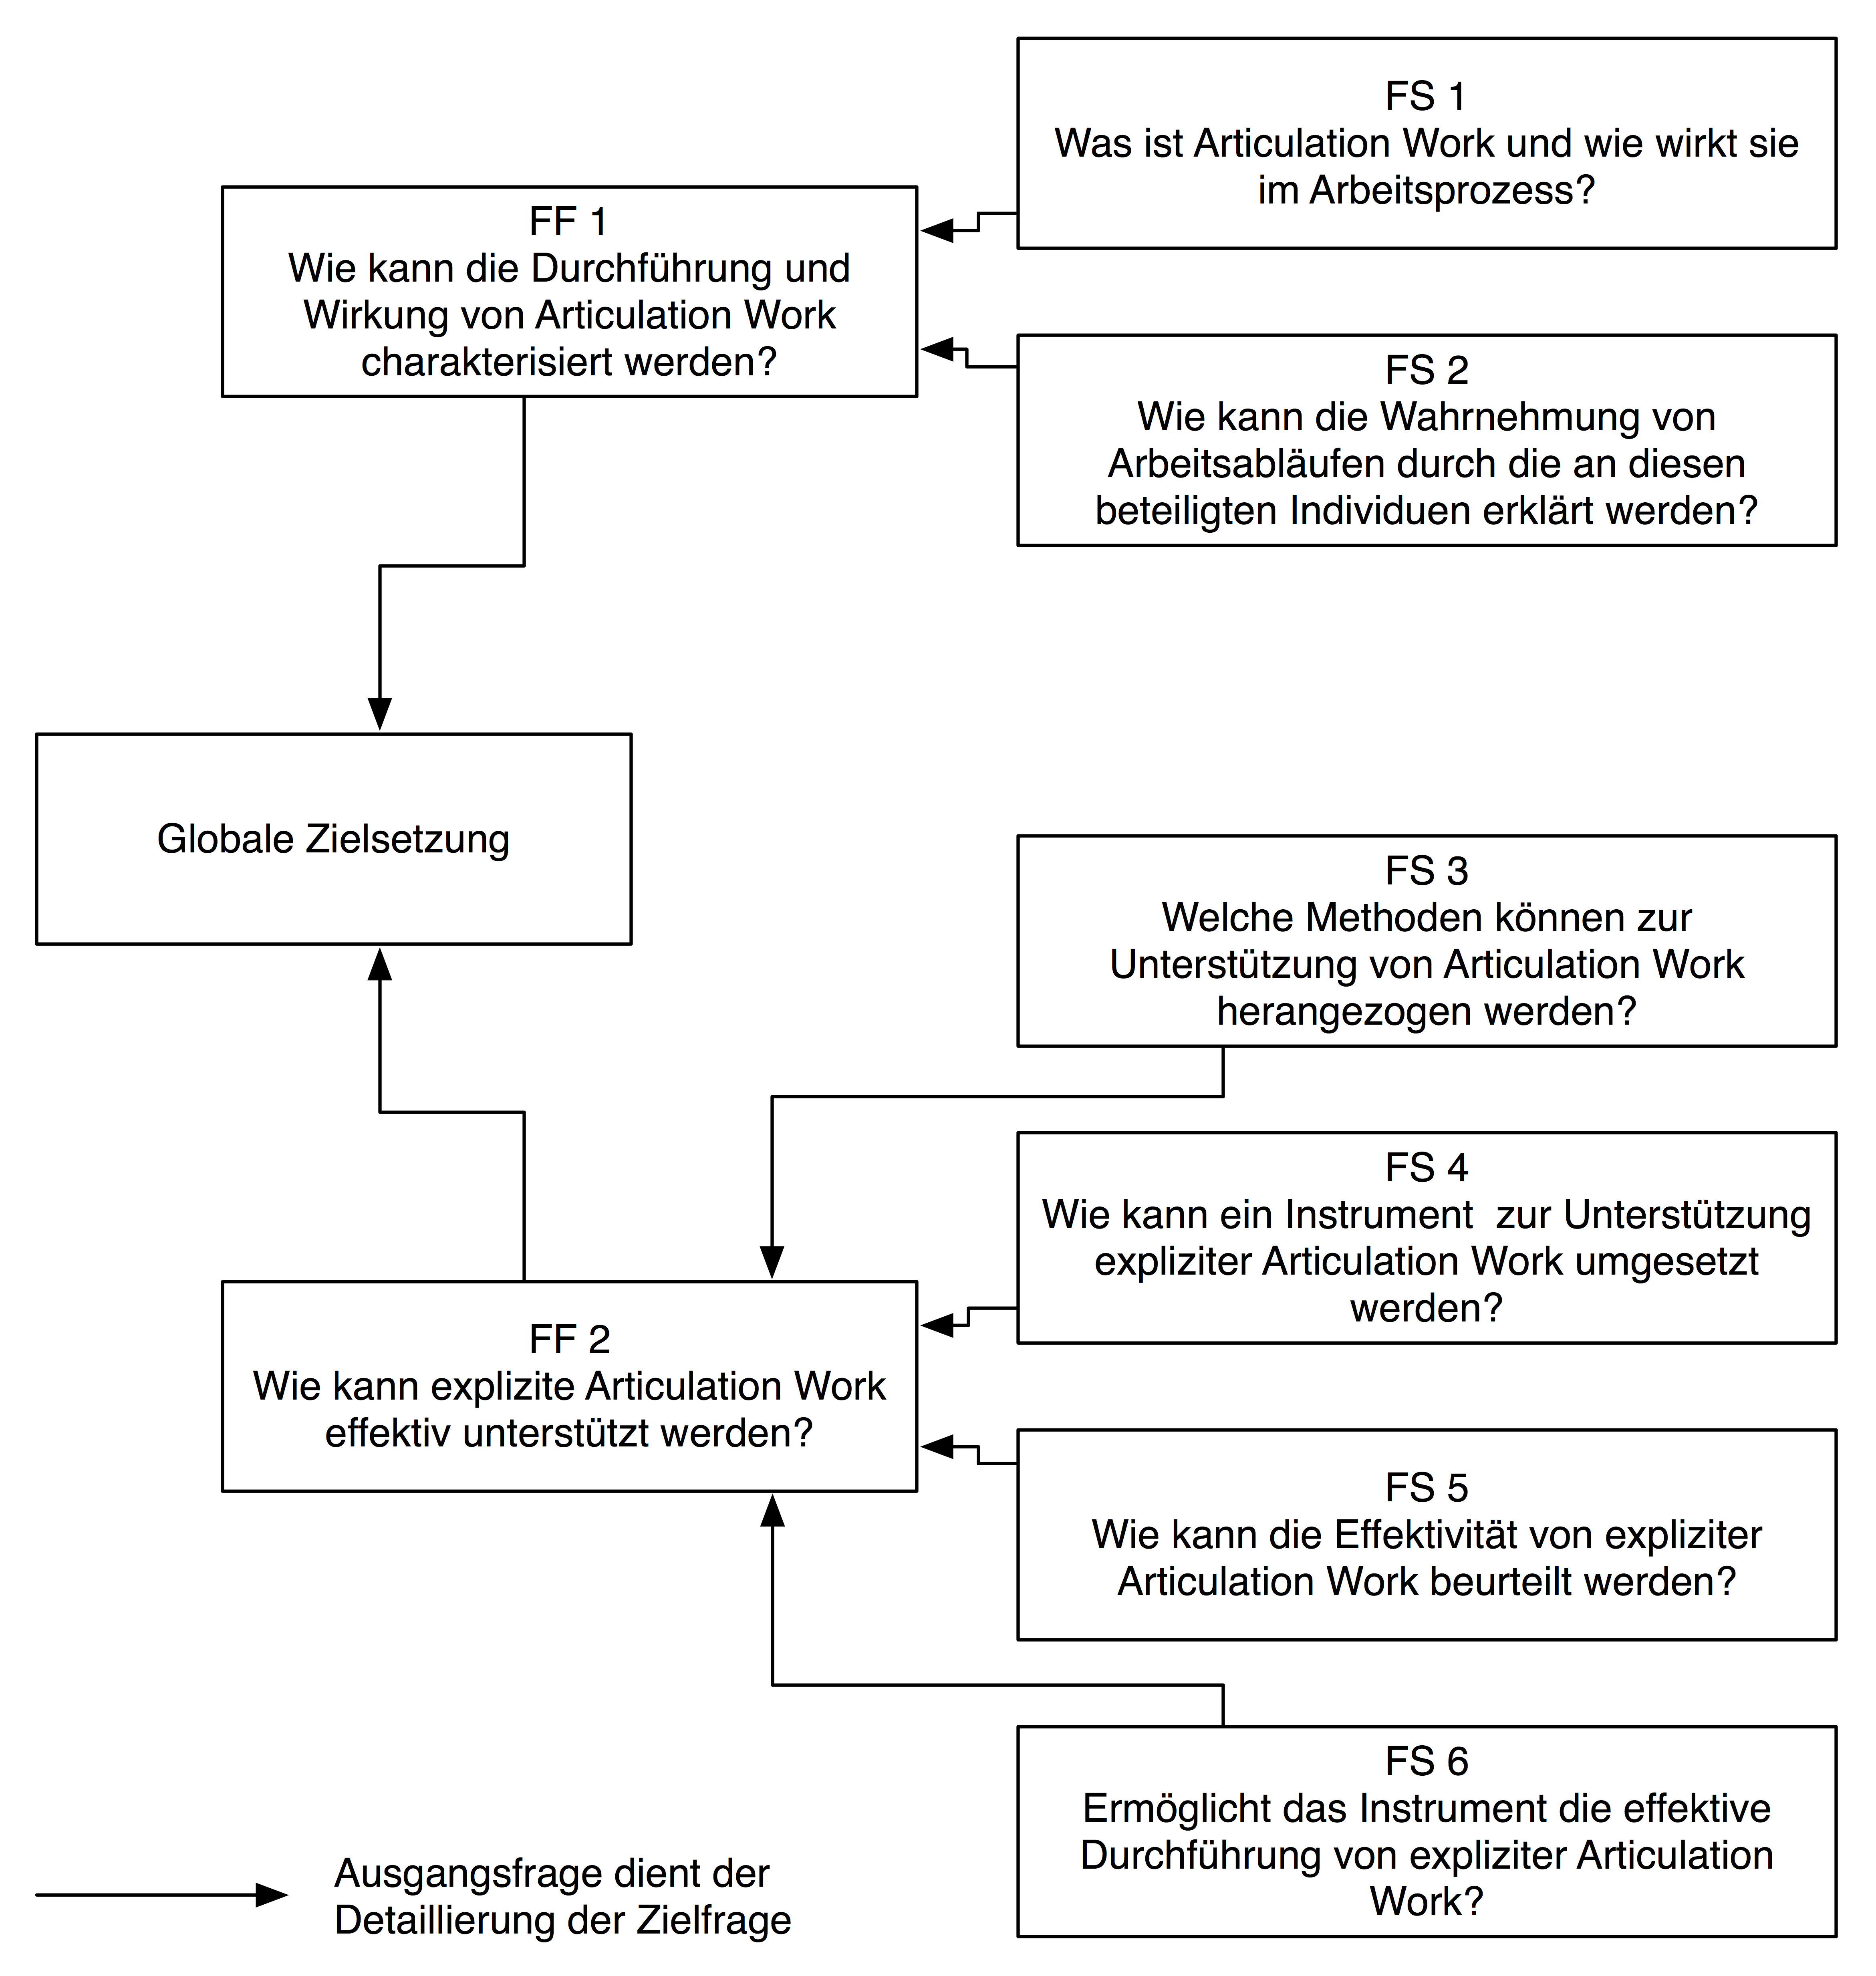
\includegraphics[width=0.9\textwidth]{img/Einfuehrung/zielhierarchie.png}
	\caption{Forschungsfragen und Fragestellungen}
	\label{fig:img_Einfuehrung_zielhierarchie}
\end{figure}

Diese Fragestellungen müssen im Rahmen der Durchführung dieser Arbeit beantwortet werden. Dazu wird in der Zusammenfassung jedes Kapitels auf diese Fragen referenziert und der jeweilige Beitrag zu deren Beantwortung identifiziert. In den Schlussbetrachtungen in Kapitel \ref{cha:schlussbetrachtungen} ist die globale Zielsetzung schließlich wieder aufzugreifen und einer abschließenden Bewertung hinsichtlich ihrer Erfüllung zu unterziehen. 

% section forschungsfragen (end)

% chapter einführung (end)
\section{Aufbau der Arbeit} % (fold)
\label{sec:aufbau_der_arbeit}

In diesem Abschnitt wird die Struktur der Arbeit auf globaler Ebene dargestellt. Zusätzlich wird der inhaltliche Aufbau der einzelnen Kapitel zueinander in Beziehung gesetzt und so der rote Faden durch die Arbeit transparent gemacht.

Die hier vorgestellte Struktur ist auszugsweise auch am Beginn jedes Kapitels beschrieben und graphisch dargestellt, um die Einordnung der Kapitel in den Gesamtzusammenhang der Arbeit zu erleichtern.

\subsection{Überblick} % (fold)
\label{sub:aufbau_ueberblick}

Die Arbeit gliedert sich inhaltlich in drei große Teile, die durch das Einleitungs- und Schlusskapitel eingerahmt werden.

Teil \ref{prt:grundlagen} behandelt die der Unterstützung von „Articulation Work“ zugrunde liegenden Forschungsgebiete und erfasst die in diesen vorgeschlagenen konkreten Maßnahmen und Methoden zur Unterstützung. Der Teil deckt damit die Beantwortung der ersten oben formulierten Forschungsfrage ab und trägt durch die Betrachtung des methodischen Teils der Unterstützung bereits zur Beantwortung der Forschungsfrage 2 bei. Im Einzelnen umfasst Teil \ref{prt:grundlagen} ein Kapitel über „Articulation Work“ (Fragestellung 1, Kapitel \ref{cha:articulation_work}) und ein Kapitel über „Mentale Modelle“ (Fragestellung 2, Kapitel \ref{cha:mentale_modelle}). Teil \ref{prt:grundlagen} endet mit einem Kapitel über Methodik der Anwendungsszenarien, in dem beschrieben wird, wie mentale Modelle für die Verwendung für „Articulation Work“ externalisiert und abgestimmt werden können und trägt damit bereits zur Forschungsfrage 2 bei (Fragestellung 3, Kapitel \ref{cha:methodik}).

Teil \ref{prt:umsetzung} behandelt die Umsetzung des Werkzeugs selbst. Er trägt damit wesentlich zur Beantwortung der zweiten oben formulierten Forschungsfrage bei, indem er das bislang auf methodischer Ebene beschriebene Unterstützungsinstrument technisch vervollständigt. Das erste Kapitel greift die Ergebnisse des ersten Teils auf und leitet daraus die Anforderungen an das Werkzeug ab (Teil der Beantwortung der Fragestellung 4, Kapitel \ref{cha:anforderungen}). In Kapitel \ref{cha:implementierung_Überblick} werden die konzeptuellen Grundlagen für die Implementierung aus dem Kontext von Tangible Interfaces heraus aufgearbeitet. Die Kapitel \ref{cha:input_&_interpretation}, \ref{cha:visualisierung} und \ref{cha:persistierung} beschreiben nacheinander die technische Umsetzung des Werkzeugs -- beginnend von den Eingabekanälen über die Ausgabekanäle bis zu Persistierung der Modelle. Sie beantworten also die Fragestellung 4. 

Teil \ref{prt:evaluierung} behandelt die Evaluierung des Werkzeugs. Er deckt damit im Wesentlichen den zweiten Teil der zweiten Forschungfrage ab, klärt das Konzept der „effektiven Unterstützung von Articulation Work“ und prüft diese für das entwickelt Instument. Dabei beginnt Kapitel \ref{cha:konzeptuelle_evaluierung} mit einer konzeptuellen Betrachtung des umgesetzten Systems (also einer theoretischen Einordnung des Werkzeugs auf Basis der Ergebnisse von Kapitel \ref{cha:implementierung_Überblick}, den konzeptuellen Grundlagen der Implementierung). In Kapitel \ref{cha:eval_ueberblick} werden die grundsätzliche Ausrichtung der empirischen Untersuchung und die durchgeführten Evaluierungen beschrieben. Die Kapitel \ref{cha:eval_werkzeug}, \ref{cha:eval_modell} und \ref{cha:eval_aw} beschäftigen sich mit der Ableitung der Hypothesen und deren Prüfung auf den unterschiedlichen Untersuchungsebenen der Arbeit. Dies beginnt mit der Prüfung der grundsätzlichen Verwendbarkeit des Systems (Kapitel \ref{cha:eval_werkzeug}), setzt mit der Prüfung der Eignung für die Externalisierung mentaler Modelle fort (Kapitel \ref{cha:eval_modell}) und endet mit der Prüfung der Eignung für „Articulation Work“ selbst (Kapitel \ref{cha:eval_aw}).

In der Zusammenfassung jedes Kapitels wird auf die betroffenen Fragestellung referenziert und der jeweilige Beitrag zur Erreichung der globalen Zielsetzung identifiziert. Der Schlussteil (Kapitel \ref{cha:schlussbetrachtungen}) fasst die Ergebnisse der Arbeit nochmals zusammen und spiegelt diese in ihrer Gesamtheit auf die ursprüngliche Zielsetzung zurück.

Die Gesamtstruktur dieser Arbeit ist in Abbildung \ref{fig:img_Einfuehrung_gesamtueberblick} nochmals zusammenfassend dargestellt. Die Beziehungen zwischen den einzelnen Kapiteln sind als Pfeile zwischen den einzelnen Blöcken dargestellt, wobei jeweils der Endpunkt Ergebnisse des Startpunktes als Grundlage für die weiteren Ausführungen verwendet.

\begin{figure}[htbp]
	\centering
		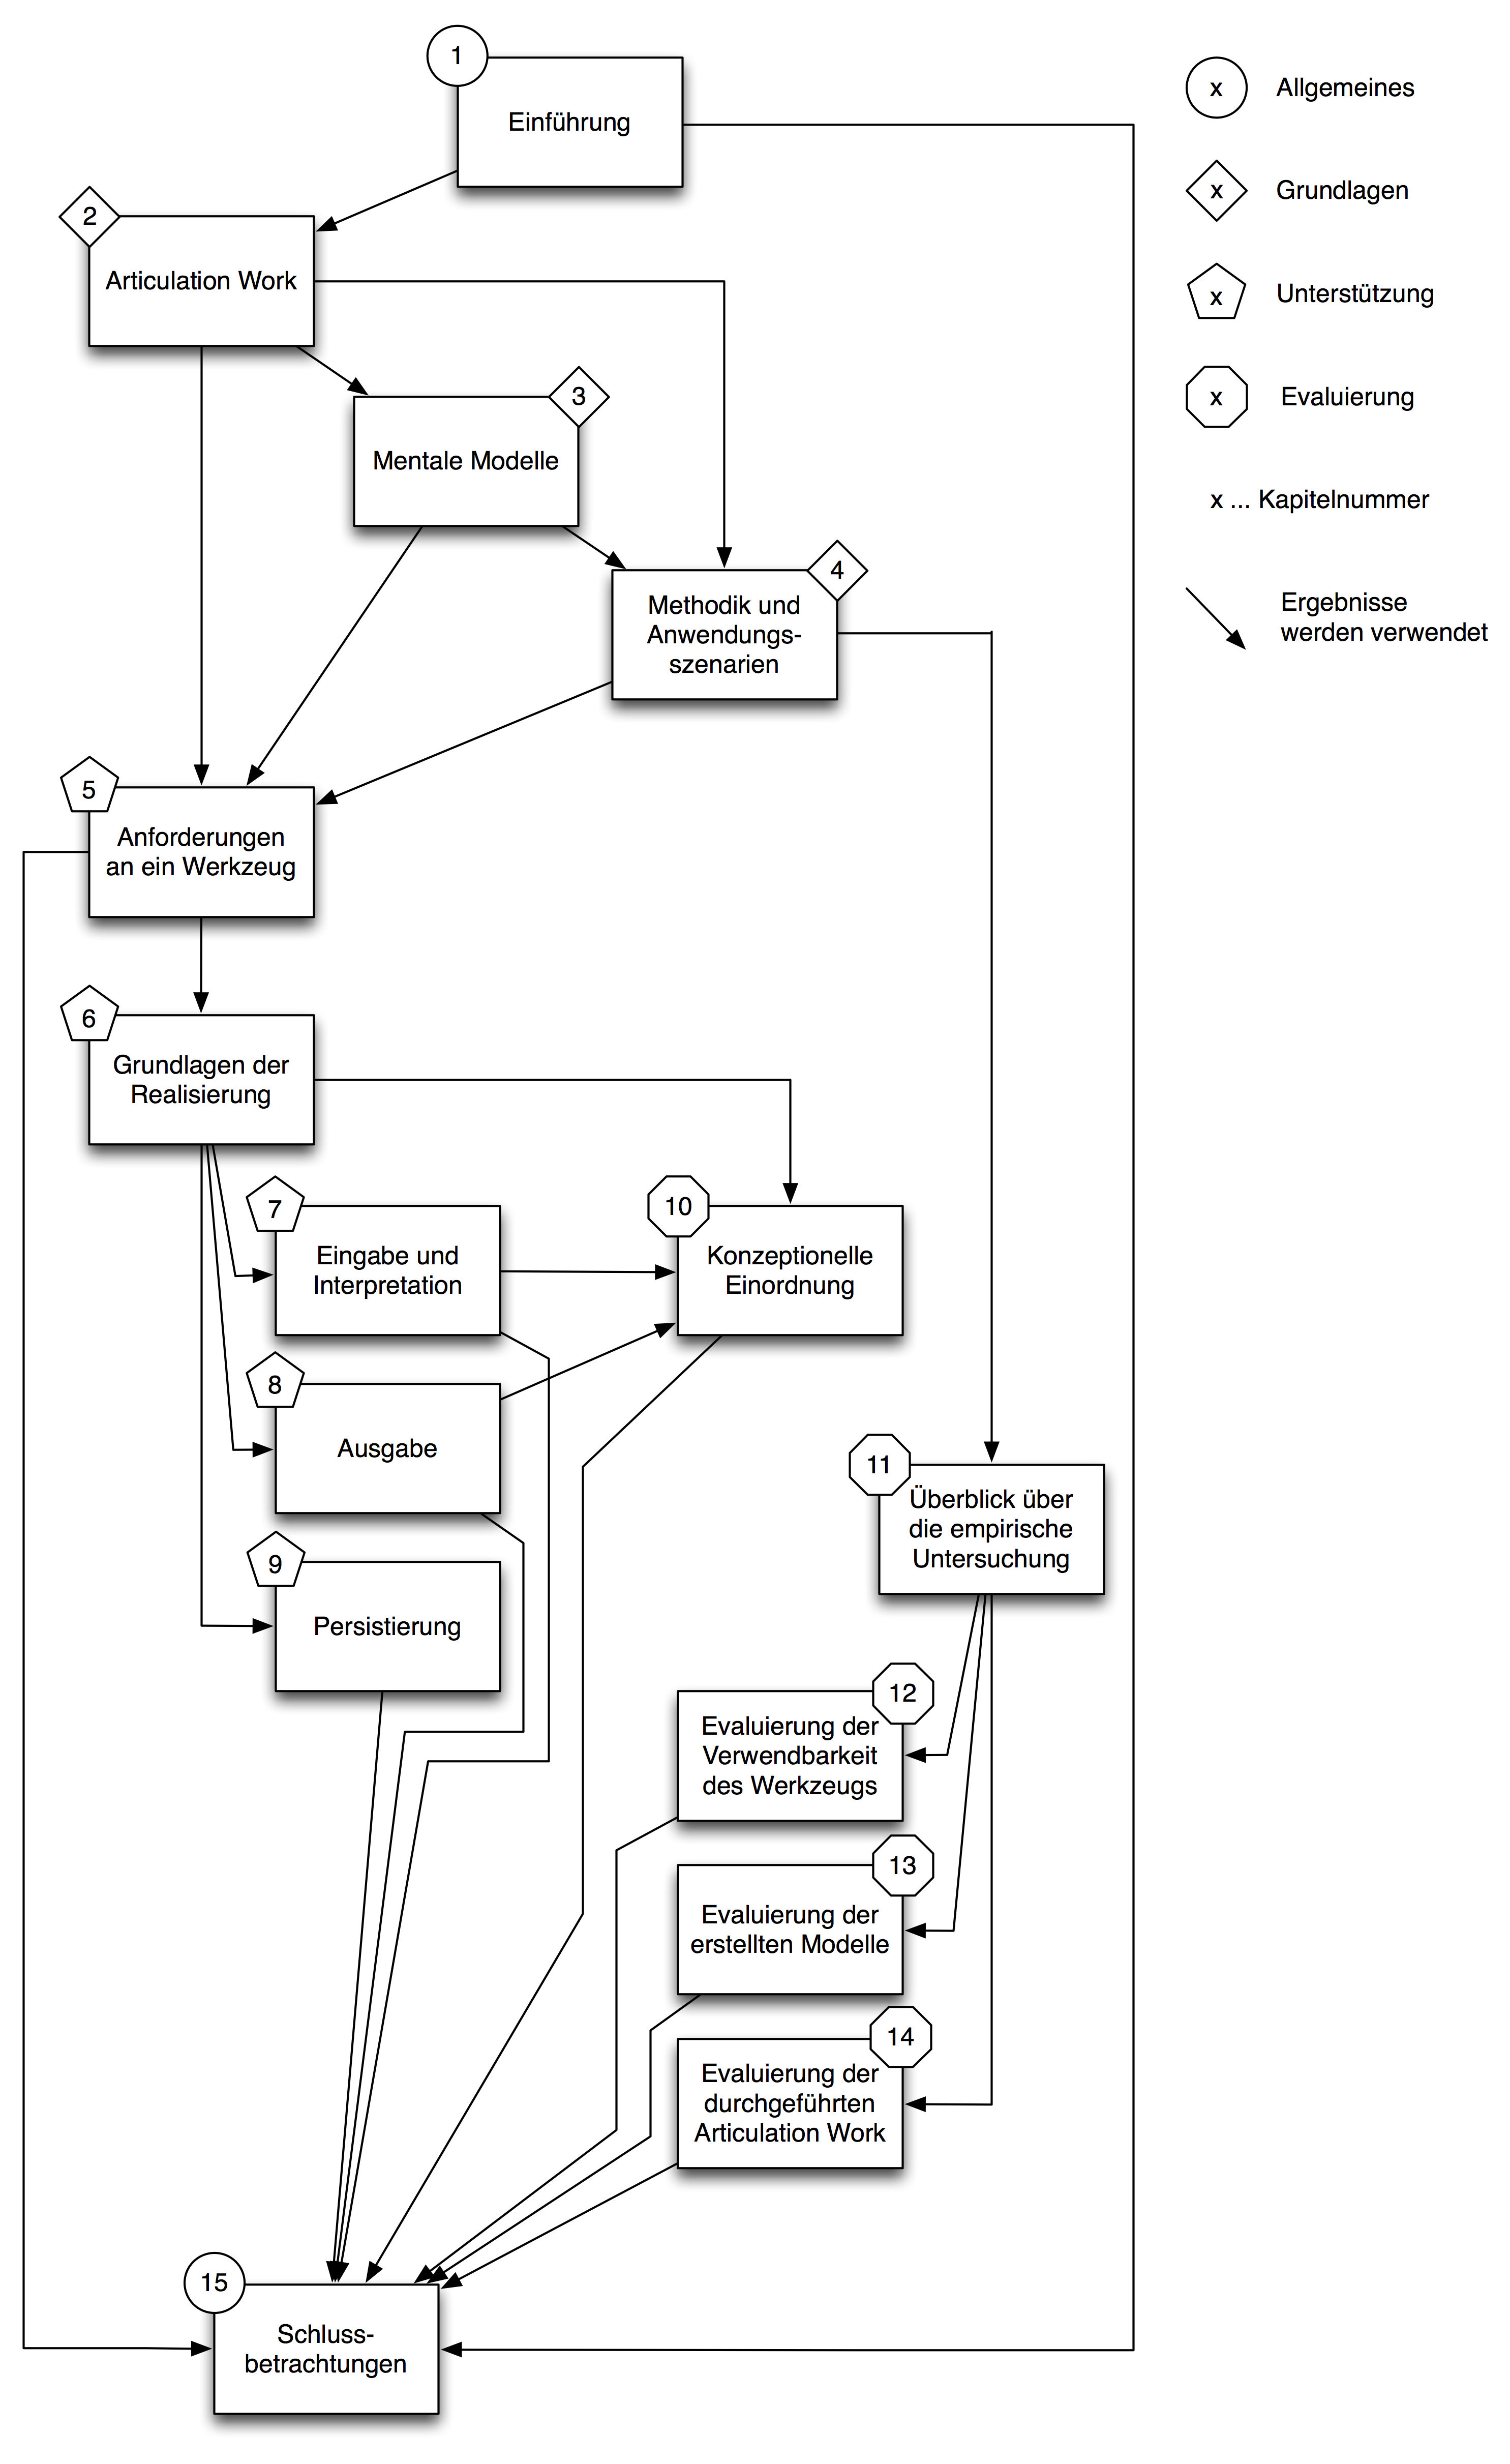
\includegraphics[height=0.9\textheight]{img/Einfuehrung/gesamtueberblick.png}
	\caption{Zusammenhänge zwischen den Kapiteln der Arbeit}
	\label{fig:img_Einfuehrung_gesamtueberblick}
\end{figure}

Anhang \ref{cha:literatur_zum_themengebiet_articulation_work} ist als Ergänzung zu Kapitel \ref{cha:articulation_work} (Articulation Work) zu sehen und stellt die gesamte zu diesem Gebiet erschienene Literatur strukturiert dar.

Anhang \ref{cha:daten_der_empirischen_untersuchung} ergänzt die Evaluierungskapitel in Teil \ref{prt:evaluierung} durch eine Zusammenfassung der im Rahmen der Untersuchung erhobenen Daten.
% subsection aufbau_ueberblick (end)

\subsection{Zusammenfassung der Zusammenhänge} % (fold)
\label{sub:zusammenhänge}

Dieser Abschnitt stellt die wesentlichen inhaltlichen Zusammenhänge der Arbeit dar und vermittelt so ein erstes Bild des roten Fadens durch die Arbeit. Er ergänzt somit die im letzten Abschnitt dargestellte Struktur der Arbeit um eine detaillierte inhaltliche Sicht und fasst das Vorgehen bei der Bearbeitung der in Abschnitt \ref{sec:forschungsfragen} formulierten Forschungsfragen zusammen.

Kapitel \ref{cha:articulation_work} beginnt mit einer generellen Begriffsbestimmung zum Themenfeld „Articulation Work“. Diese bildet die Grundlage für den nächsten Abschnitt, in dem auf Basis der Literatur geklärt wird, wie sich „Articulation Work“ manifestiert und in welchen unterschiedlichen Ausprägungen sie das tut. Das Ergebnis ist in Abbildung \ref{fig:img_ArticulationWork_aw_conceptual_structure} zusammengefasst und spannt die in dieser Arbeit verwendete Taxonomie auf. In den beiden folgenden Abschnitten wird auf Basis der Literatur dargestellt, was (welche Arbeitsaspekte) Gegenstand von „Articulation Work“ ist und wie „Articulation Work“ unterstützt werden kann (siehe dazu auch Anhang \ref{cha:literatur_zum_themengebiet_articulation_work} für eine Gesamtübersicht über die zu „Articulation Work“ verfügbare Literatur). Schließlich greift der letzte Abschnitt die Ergebnisse der Literaturstudien wieder auf und identifiziert eine konzeptuelle Lücke bei der Betrachtung von kooperativer Arbeit anhand der Theorie von Strauss, die auch schon im Rahmen der Einleitung identifiziert wurde  -- nämlich die bislang vernachlässigte Rolle des Individuums bei „Articulation Work“ und dessen konkrete Tätigkeiten. Zu diesem Aspekt existieren wenige Aussagen in der Literatur zu „Articulation Work“, \citet{Strauss93} selbst weist jedoch darauf hin, dass eine konzeptuelle Lücke entsteht, wenn auf die sozialen und organisationalen Aspekte von „Articulation Work“ fokussiert wird, die individuellen „thought processes“ aber außer Acht gelassen werden.

In Kapitel \ref{cha:mentale_modelle} wird die identifizierte Lücke aufgegriffen und konzeptuell mit dem Erklärungsmodell der mentalen Modelle \citep{Johnson-Laird81} hinterlegt. Im Kontext von „Articulation Work“ sind mentale Modelle jener Beitrag, den jedes beteiligte Individuum einbringt und der in der Folge Gegenstand der Abstimmung und Aushandlung sein muss, um eine gemeinsame Sichtweise zu entwickeln und „contingencies“ aufzulösen (was letztendlich das Ziel von „Articulation Work“ ist \citep{Gerson86}). Dementsprechend beschäftigt sich der nächste Abschnitt mit der Bildung und Veränderung mentaler Modelle, wobei als wesentliches Hilfsmittel dazu die Externalisierung derselben identifiziert wird \citep{Seel91}. Zur Externalisierung werden drei in der Literatur genannte Ansätze vorgestellt \citep{Ifenthaler06}. Diesen sind Strukturlegetechniken \citep{Dann92} sowie Concept Mapping \citep{Novak06} zuzurechnen, die in der Folge durch ihre kooperative Anwendbarkeit als die für „Articulation Work“ am besten geeigneten Ansätze identifiziert werden (vor allem Strukturlegetechniken unterstützen inhärent den Abstimmungsprozess von mentalen Modellen \citep{Groeben00}).

Dies führt zu Kapitel \ref{cha:methodik}, in dem auf Basis der beiden Ansätze die Methoden zur Externalisierung von mentalen Modellen beschrieben werde. Diese werden den Eigenschaften von „Articulation Work“ gegenüber gestellt und daraus ein Vorgehen abgeleitet, dass Strukturlegetechniken und Concept Mapping in einer Methodik zusammenführt. Diese Methodik soll möglichst offen (im Sinne von prozedural und inhaltlich flexibel) die Externalisierung und Abstimmung mentaler Modelle ermöglichen. Der zweite Teil des Kapitels stellt mögliche Anwendungsszenarien vor, die im Kontext von „Articulation Work“ auftreten können. Diese Anwendungsszenarien schlagen die Brücke zu den Anwendungen im Rahmen der Evaluierung (siehe Kapitel \ref{cha:eval_ueberblick}), da diese den einzelnen Evaluierungsteilen zugeordnet werden können.

Das Methodik-Kapitel leitet in Teil \ref{prt:umsetzung} der Arbeit über, wo die konkrete Unterstützung von „Articulation Work“ durch ein Werkzeug besprochen wird. Als Ausgangspunkt für das Kapitel \ref{cha:anforderungen} wird auf Teil \ref{prt:grundlagen} und dort speziell auf das Kapitel zur Methodik zurückgegriffen und aus den dortigen Ergebnissen Anforderungen an ein Werkzeug abgeleitet, das die vorgeschlagene Vorgehensweise unterstützt. Konzeptuell ist hier zwischen Anforderungen zu unterscheiden, die aus der Concept Mapping Methodik stammen (im Wesentlichen „Flexibilität der Repräsentation“), Anforderungen, die von Strukturlegetechniken abzuleiten sind (im Wesentlichen „Physikalität der Repräsentation“) und jenen, die direkt aus „Articulation Work“ abgeleitet werden können (im Wesentlichen „Kooperative Bedienbarkeit“).

Die Festlegung dieser Anforderungen ist die Grundlage der konkreten Umsetzung des Werkzeugs. Kapitel \ref{cha:anforderungen} endet mit der Feststellung, dass aufgrund der Anforderungen aus allen drei Bereichen ein „Tangible Tabletop Interface“ geeignet wäre, entsprechende Werkzeugunterstützung zu liefern. „Tangible“ motiviert sich dabei aus der in Strukturlegetechniken geforderten Physikalität der Abbildung, „Tabletop“ aus der unmittelbaren kooperativen Bearbeitbarkeit, die durch „Articulation Work“ selbst gefordert wird und „Interface“ (in diesem Kontext ist darunter die Rechnerunterstützung zu verstehen) durch die im Rahmen von Concept Mapping vorgeschlagenen Maßnahmen zur Modellierungsunterstützung, die nur durch Funktionen im Rechner realisiert werden können.

Vor der konkreten Umsetzung geht das folgende Kapitel (Kapitel \ref{cha:implementierung_Überblick}) detailliert auf die Thematik der „Tangible Tabletop Interfaces“ ein. Neben einem historischen Überblick schlägt Abschnitt \ref{sec:lernprozesse_und_tangible_interface} ausgehend von der eher technologiezentrierten Sichtweise der „Tangible Interface“-Forschung die Brücke zurück zu den mentalen Modellen und Lernprozessen, die in Kapitel \ref{cha:mentale_modelle} („Mentale Modelle“) besprochen wurden. Einige der genannten Aspekte lassen sich auch auf die Anforderungen von „Articulation Work“ abbilden, was im zweiten Teil dieses Abschnitts beschrieben wird. Als zweiten Brückenschlags in den Grundlagenteil wird die Forschung zu den Auswirkungen von „Tangible Interfaces“ auf die Kooperation der Anwender betrachtet -- ein Bereich der unmittelbar für „Articulation Work“ selbst relevant ist und damit die Brücke zurück zu Kapitel \ref{cha:articulation_work} schlägt. Mit diesen beiden Abschnitten (\ref{sec:lernprozesse_und_tangible_interface} und \ref{sec:kooperation_und_tangible_interfaces}) wird nochmals (aus „technischer“ Sicht) begründet, das „Tangible Interfaces“ für den geplanten Anwendungsbereich (kooperative Externalisierung und Abstimmung mentaler Modelle) geeignet sind.

Der zweite Teil von Kapitel \ref{cha:implementierung_Überblick} (ab Abschnitt \ref{sec:konzeptualisierungen_von_tangible_interfaces}) beschäftigt sich mit Ansätzen, „Tangible Interfaces“ konzeptuell zu betrachten. Dazu wird die existierende Literatur umfassend aufgearbeitet und strukturiert dargestellt. Dieser Teil wird in Kapitel \ref{cha:konzeptuelle_evaluierung} wieder aufgegriffen und zur Einordnung des entwickelten Systems in den Designraum der „Tangible Interface“-Forschung verwendet. Auch in den Kapiteln \ref{cha:input_&_interpretation} und \ref{cha:visualisierung}, die die konkrete Umsetzung des Werkzeugs beschreiben, wird auf einzelne dieser konzeptuellen Erklärungsmodelle zurückgegriffen, die explizit für die Unterstützung der Konzeption von Tangible Interfaces entwickelt wurden.

Teil 3 von Kapitel \ref{cha:implementierung_Überblick} wird wieder konkreter und engt den Betrachtungsbereich von „Tangible Interfaces“ auf „Tabletop Interfaces“ ein, um letztendlich auf „Tabletop Interfaces zur Erstellung diagrammatischer Modelle“ zu fokussieren, was im Wesentlichen die unmittelbare „Related Work“ zu der vorliegenden Arbeit aus technischer Sicht darstellt. Auch dazu wird jeweils die verfügbare Literatur (aus historischer Sicht sowie den „State of the Art“) aufgearbeitet.

Nach diesem umfassenden Überblickskapitel behandeln die Folgekapitel die konkrete technische Umsetzung des Werkzeugs. Das Werkzeug wurde dazu konzeptuell in drei Blöcke unterteilt. Kapitel \ref{cha:input_&_interpretation} beschäftigt sich mit der Eingabe von Information über das „Tabletop Interface“ und der Aufbereitung und Interpretation der Eingabedaten für den spezifischen Anwendungsfall (also der „Modellierung“). Dabei erfolgt die Beschreibung vom Allgemeinen ins Spezielle und beginnt mit der Darstellung der grundlegenden Möglichkeiten, auf einem „Tabletop Interface“ Benutzereingaben zu ermöglichen. Auf Basis der Anforderungen aus Kapitel \ref{cha:anforderungen} wird eine Technologieentscheidung getroffen (optische Erkennung der Bausteine). Dazu werden in der Folge die in diesem Bereich verfügbaren Softwareframeworks dargestellt und wiederum strukturiert gegenübergestellt. Die folgende Framework-Entscheidung für das ReacTIVision-System \citep{Kaltenbrunner07} ermöglicht die Festlegung des konkrete Hard- und Softwaredesign für die Erkennung von Benutzereingaben. In den folgenden Abschnitten wird die Implementierung beginnend von der Benutzungsschnittstelle (in diesem Fall Hardware) hin zur Richtung Software zur Erkennung und Interpretation der Benutzereingaben dargestellt. Nach der Beschreibung der Hardware in Abschnitt \ref{sec:konzeption_und_umsetzung_der_hardwarekomponenten} wird in Abschnitt \ref{sec:benutzerinteraktion_mit_dem_werkzeug} die Interaktion der Benutzer mit dem Werkzeug beschrieben. Damit kommt die Anwendungssicht (also die „Modellierung“) ins Spiel, die benötigt wird, um die Interpretation der Eingabedaten zu beschreiben. Dies erfolgt in Abschnitt \ref{sec:erfassung_der_benutzerinteraktion_durch_softfware}. Das Kapitel endet an jenem Punkt, wo auch in der Software eine Schnittstelle zur Entkopplung und Modularisierung eingeführt wurde -- bei der Übergabe der interpretierten und auf Modellierungsaktivitäten abstrahierten Eingabedaten an die weiterverarbeitenden Schichten (siehe Abbildung \ref{fig:img_ImplementierungInput_InputArchitecture}).

Kapitel \ref{cha:visualisierung} widmet sich der Ausgabe und ist analog zu Kapitel \ref{cha:input_&_interpretation} aufgebaut. Beginnend von den grundsätzlichen Möglichkeiten zur Ausgabe immer weiter fokussiert, bis die konkreten Umsetzung der Informationsausgabe mittels dem JHotDraw-Framework \citep{Gamma96} dargestellt werden kann. Wo in Kapitel \ref{cha:input_&_interpretation} durch Beschreibung der Benutzerinteraktionen auf den konkreten Anwendungsfall der Technologie fokussiert wurde, wird hier zum gleichen Zweck die Beschreibung und Zuordnung der auszugebenden Information in Abschnitt \ref{sec:ausgabe_von_information} beschrieben und die Unterscheidung getroffen, ob die Ausgabe direkt auf der Tischoberfläche oder disloziert auf einer separaten Darstellungsfläche zu passieren hat. Die Feststellung, dass mehrere Ausgabekanäle benötigt werden, um die auszugebende Information darstellen zu können, führt zum konkreten Softwaredesign in Abschnitt \ref{sec:umsetzung_der_ausgabe_mit_software}. Dieses ist durch den Einsatz eines Dispatchers modular aufgebaut und erweiterbar angelegt (siehe Abbildung \ref{fig:img_ImplementierungOutput_OutputArchitecture} bzw. Abbildung \ref{fig:img_ImplementierungOutput_OutputClasses}).

In Kapitel \ref{cha:persistierung} wird die Persistierung der erstellten Modelle und der gewonnenen Metainformation besprochen. Dazu identifiziert der einleitende Abschnitt auf Basis der Notwendigkeit einer flexiblen Repräsentationsform „Topic Maps“ \citep{TMDM08} als ein geeignetes Mittel für die Abbildung. In der Folge wird  wieder auf den konkreten Anwendungsfall eingegangen. Nach der Beschreibung von „Topic Maps“ wird die Abbildung der erstellten Modelle auf „Topic Maps“ und letztendlich die konkrete Implementierung der Persistierung dargestellt. Abschnitt \ref{sec:export_graphischer_repräsentationen} stellt die unterschiedlichen Möglichkeiten zum graphischen Export der Modelle dar, der für die unmittelbare Dokumentation des Modellierungsprozesses und -ergebnisses notwendig ist. Dieses Kapitel schließt Teil \ref{prt:umsetzung} der Arbeit ab.

In Teil \ref{prt:evaluierung} wird die Evaluierung des Werkzeugs behandelt. Dies beginnt mit der konzeptuellen Einordnung des erstellten Werkzeugs. Dazu werden sämtliche Ansätze zur Konzeptualisierung von Tangible Interfaces aus Abschnitt \ref{sec:konzeptualisierungen_von_tangible_interfaces} herangezogen und das Werkzeug in seiner aktuellen Implementierung in diese eingeordnet. Das Ziel ist dabei einerseits, das Werkzeug in die bisherige Forschung einzuordnen, andererseits aber auch etwaiges Verbesserungspotential zu identifizieren, das etwa durch Inkonsistenzen der Ausprägungen innerhalb der jeweiligen Betrachtungsdimensionen aufgedeckt werden kann. Während die Einordnung in allen 12 betrachteten Ansätzen möglich ist, kann Verbesserungspotential nur in 7 Ansätzen identifiziert werden. In der Zusammenfassung des Kapitels wird einerseits die Eignung eines Ansatzes zur Einordnung des vorliegenden Systems und der ggf. entstehenden Mehrwert besprochen. Andererseits wird das Verbesserungspotential aufgezeigt, das sich aus der rein konzeptuellen Betrachtung des Systems ableiten lässt. Im Rahmen der empirischen Untersuchung in den folgenden Kapiteln werden diese Punkte aufgegriffen und hinsichtlich ihrer tatsächlich in der Praxis aufgetretenen Relevanz betrachtet.

Die Kapitel \ref{cha:eval_ueberblick} bis \ref{cha:eval_aw} beschreiben die empirische Untersuchung. Kapitel \ref{cha:eval_ueberblick} ist dabei wiederum als Übersichtskapitel konzipiert. Dort werden die zu untersuchenden Aspekte aus der Zielsetzung abgeleitet und die Einteilung in die Kapitel \ref{cha:eval_werkzeug} bis \ref{cha:eval_aw} argumentiert. Untersuchungen werden auf Ebene des Werkzeugs (Benutzbarkeit), der „Mentalen Modelle“ (Eignung des Werkzeugs zur Externalisierung) sowie von „Articulation Work“ selbst (Unterstützung des Aushandlungsprozesses) durchgeführt. Für jeden dieser Blöcke wird eingeführt, auf Basis welcher Literatur die Untersuchung angelegt werden kann. In der darauf folgenden Beschreibung des globalen Untersuchungsdesigns werden alle durchgeführten Untersuchungen vorgestellt. Diese Vorstellung umfasst den Anwendungskontext, die Aufgabenstellung sowie die Beschreibung der Teilnehmer bzw. deren Hintergrund. Die Zuordnung zwischen den Untersuchungen und den untersuchten Aspekten erfolgt im Rahmen der Vorstellung der jeweiligen Untersuchung und zusammengefasst nochmals im letzen Abschnitt des Kapitels. Nach der Vorstellung der Untersuchungen werden die eingesetzten empirischen und statistischen Methoden beschrieben, auf die in den Kapiteln \ref{cha:eval_werkzeug} bis \ref{cha:eval_aw} nur noch namentlich verwiesen wird.

Die Kapitel \ref{cha:eval_werkzeug} bis \ref{cha:eval_aw} widmen sich der Prüfung der drei identifizierten Untersuchungsebenen. Alle drei Kapitel sind identisch aufgebaut. Im jeweils ersten Abschnitt werden die zu prüfenden Hypothesen abgeleitet. Diese Ableitung erfolgt aus der Zielsetzung, hinterlegt mit den konzeptuellen Grundlagen der Arbeit aus Teil \ref{prt:grundlagen}. Zusätzlich werden explorativ gebildete Hypothesen formuliert, die nicht unmittelbar aus der Zielsetzung ableitbar sind, die aber Auffälligkeiten abbilden, die im Rahmen der ersten, explorativen Untersuchungen des Werkzeugs offensichtlich wurden und die an dieser Stelle nochmals dezidiert geprüft werden sollen, um die Vermutungen zu bestätigen oder diese  widerlegen zu können. Im auf die Formulierung der Hypothesen folgenden Abschnitt über Untersuchungsdesign und Durchführung werden einerseits die Hypothesen operationalisiert (d.h. deren konkrete Prüfung vorgestellt und argumentiert) und in der Folge die Durchführung der Untersuchungen beschrieben. An dieser Stelle wird auf die im vorhergehenden Kapitel vorgestellten Untersuchungen zurückgegriffen und der jeweils relevante Teil im Detail beschrieben. Der dritte Abschnitt jedes Kapitels präsentiert die Ergebnisse der Untersuchung. Für jede Hypothese wird die Auswertung durchgeführt, das Ergebnis diskutiert und in einem separaten Unterabschnitt nochmals zusammengefasst. Die Beschreibung der Auswertung umfasst dabei sowohl quantitative Daten (z.T. graphisch aufbereitet) als auch qualitative Ergebnisse, die meist in der Form von Transkripten von Auszügen aus Modellierungsprozessen eingefügt werden.

In den Schlussbetrachtungen in Kapitel \ref{cha:schlussbetrachtungen} werden die Ergebnisse der Evaluierung zusammengefasst und auf Anforderungen an das Werkzeug sowie die globale Zielsetzung rückgespiegelt. Aufbauend darauf werden weitere Entwicklungsmöglichkeiten des Werkzeugs aufgezeigt und weiterführende Anwendungsszenarien beschrieben. Eine Reflexion des gesamten Entstehungsprozesses schließt diese Arbeit ab.

Abbildung \ref{fig:img_Einfuehrung_zusammenhang} stellt die Bezüge zwischen den Kapitel und den zu bearbeitenden Fragestellungen nochmals graphisch dar. Die hier abgebildeten Bezüge werden auch in den Zusammenfassungen der jeweiligen Kapitel beschrieben und inhaltlich argumentiert.

\begin{figure}[htbp]
	\centering
		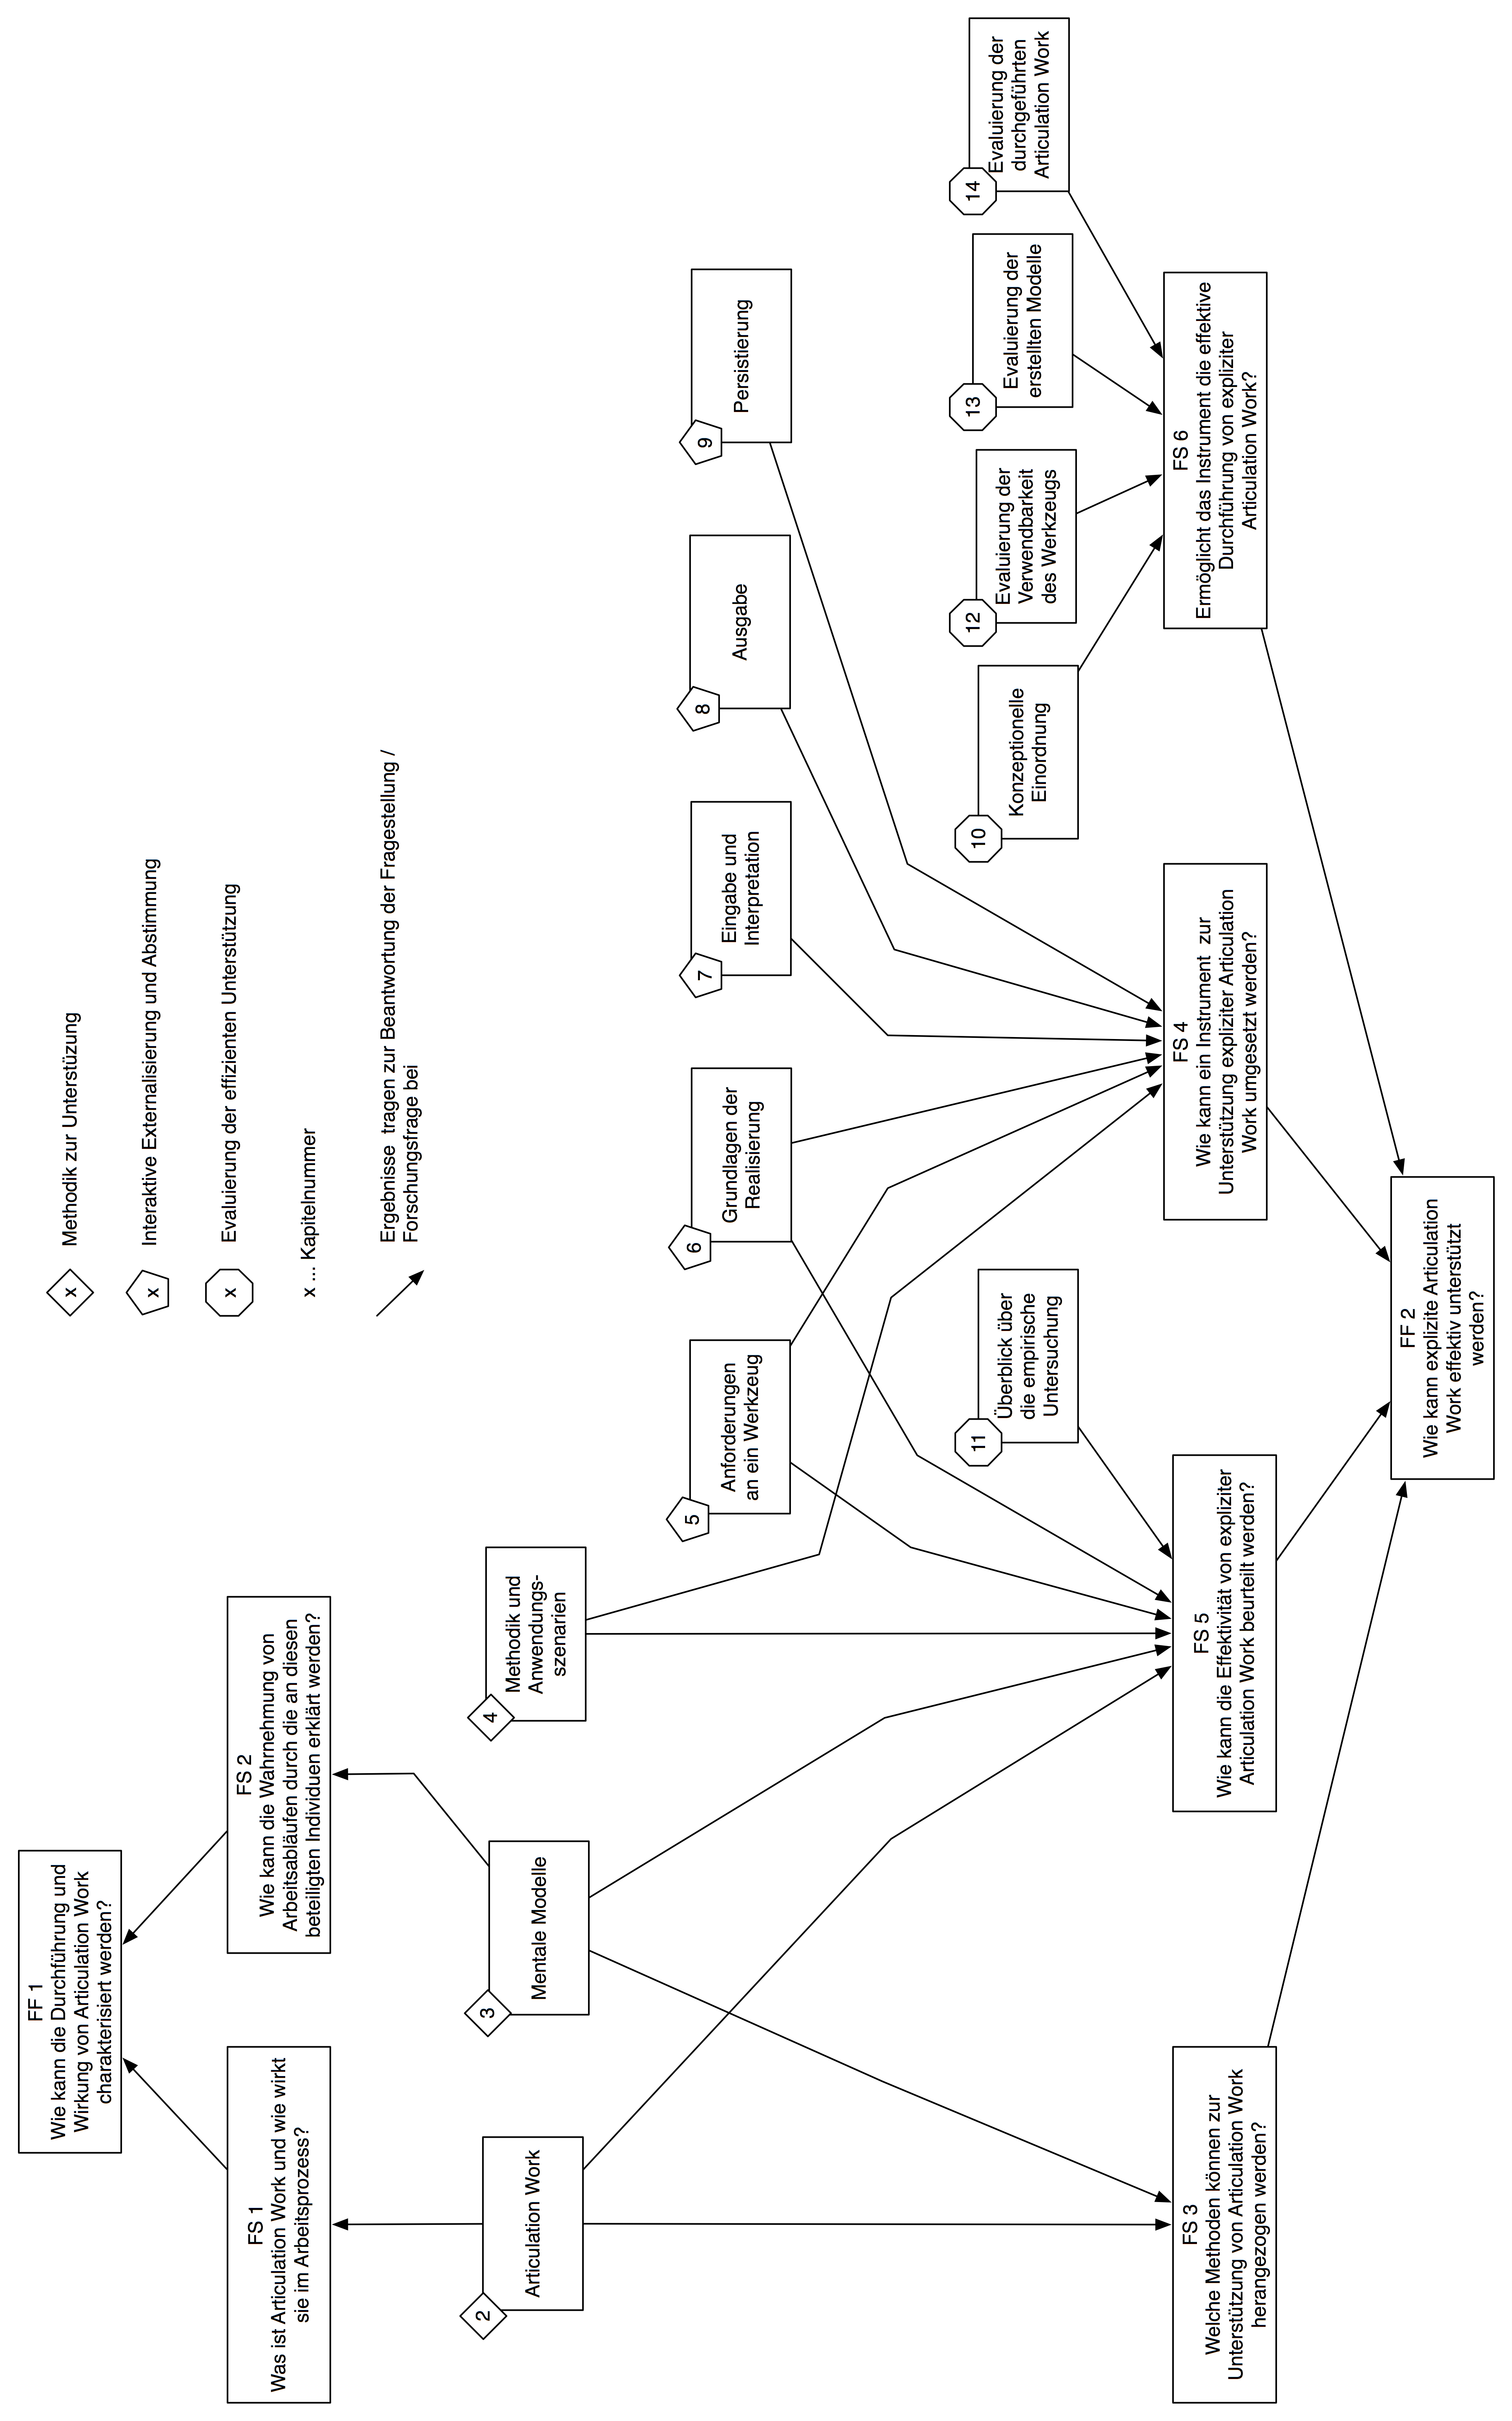
\includegraphics[height=.9\textheight]{img/Einfuehrung/zusammenhang.png}
	\caption{Zusammenhang zwischen Zielsetzung und Struktur der Arbeit }
	\label{fig:img_Einfuehrung_zusammenhang}
\end{figure}


% subsection zusammenhänge (end)
% section aufbau_der_arbeit (end)


\chapter{Articulation Work} % (fold)
\label{cha:articulation_work}

In diesem Kapitel wird das Konzept „Articulation Work“ dargestellt und in den Kontext von menschlicher Arbeit an sich gestellt. Der zweite Teil des Kapitels widmet sich den Aktivitäten, die „Articulation Work“ ausmachen, den Merkmalen, an denen sich gute „Articulation Work“ zeigt, sowie den Möglichkeiten der Unterstützung von „Articulation Work“ durch organisationale und technische Maßnahmen.

\section{Begriffsbestimmung} % (fold)
\label{sec:aw_begriffsbestimmung}

Das Konzept der "Articulation Work" wurde als Erklärungsmodell für einen bestimmten Typus von menschlicher Arbeit Mitte der 1980er Jahre von  \citet{Strauss85} im Kontext von Fallstudien aus der Krankenhaus-Organisation eingeführt. "Articulation Work" ist dabei jener Anteil an menschlicher Arbeit, der der Abstimmung mit anderen Individuen dient. Diese Abstimmung ist notwendig um das eigentliche Arbeitsziel erreichen zu können. Arbeit wird als inhärent kooperative Prozess gesehen, der immer auf Interaktion mit anderen Menschen basiert bzw. diese bedingt (Strauss formuliert diese Annahme in Bezugnahme auf \citet{Hughes71} prägnant mit der Aussage \emph{„work rests ultimately on interaction“}). Diese Annahme erscheint insofern als zulässig, als dass selbst Arbeitsabläufe, die selbst keine Kooperation mit anderen Menschen bedingen, zumindest auf den Ergebnissen anderer Arbeitsabläufe aufbauen oder als Grundlage weiterer Arbeitsabläufe dienen. Interaktion tritt also in jedem Arbeitsprozess zumindest zu Beginn und am Ende in unmittelbarer oder mittelbarer\footnote{Unter "mittelbar" ist hier Interaktion zu verstehen, die nicht im direkten Kontakt zwischen Individuen abläuft sondern lediglich indirekt durch die Ergebnisse eines Arbeitsprozesses (Materialien, Dokumente, \ldots) vermittelt wird.} Form auf.

\textbf{Abbildung, in der kooperative Arbeitsprozesse und solche mit mittelbarer und unmittelbarer Interaktion zu Beginn oder am Ende dargestellt werden}

Jener Teil von Arbeit, der der eigentlichen Zielerreichung dient, wird im hier vorgestellten Erklärungsmodell als „Production Work“ bezeichnet \citep{Fujimura87}. „Production Work“ ist komplementär zu „Articulation Work“ zu sehen und umfasst alle Aktivitäten, die der „Wertschöpfung“ im wörtlichen Sinn, also der Schaffung jener Werte (oder Ergebnisse), die durch den Arbeitsablauf erreicht werden sollten. Wenn hier von Arbeit bzw. Arbeitsabläufen die Rede ist, so ist darunter eine Kette von Aktivitäten zu verstehen, die der Erreichung eine vorab gewählten Ziels dient\footnote{siehe dazu etwa die Definition von Arbeit durch \citet{Semmer04}: \emph{„Arbeit ist zielgerichtete menschliche Tätigkeit zum Zwecke der Transformation und Aneignung der Umwelt aufgrund selbst- oder fremddefinierter Aufgaben, mit gesellschaftlicher, materieller oder ideeller Bewertung, zur Realisierung oder Weiterentwicklung individueller oder kollektiver Bedürfnisse, Ansprüche und Kompetenzen.“}}. 

\begin{figure}[htbp]
	\centering
		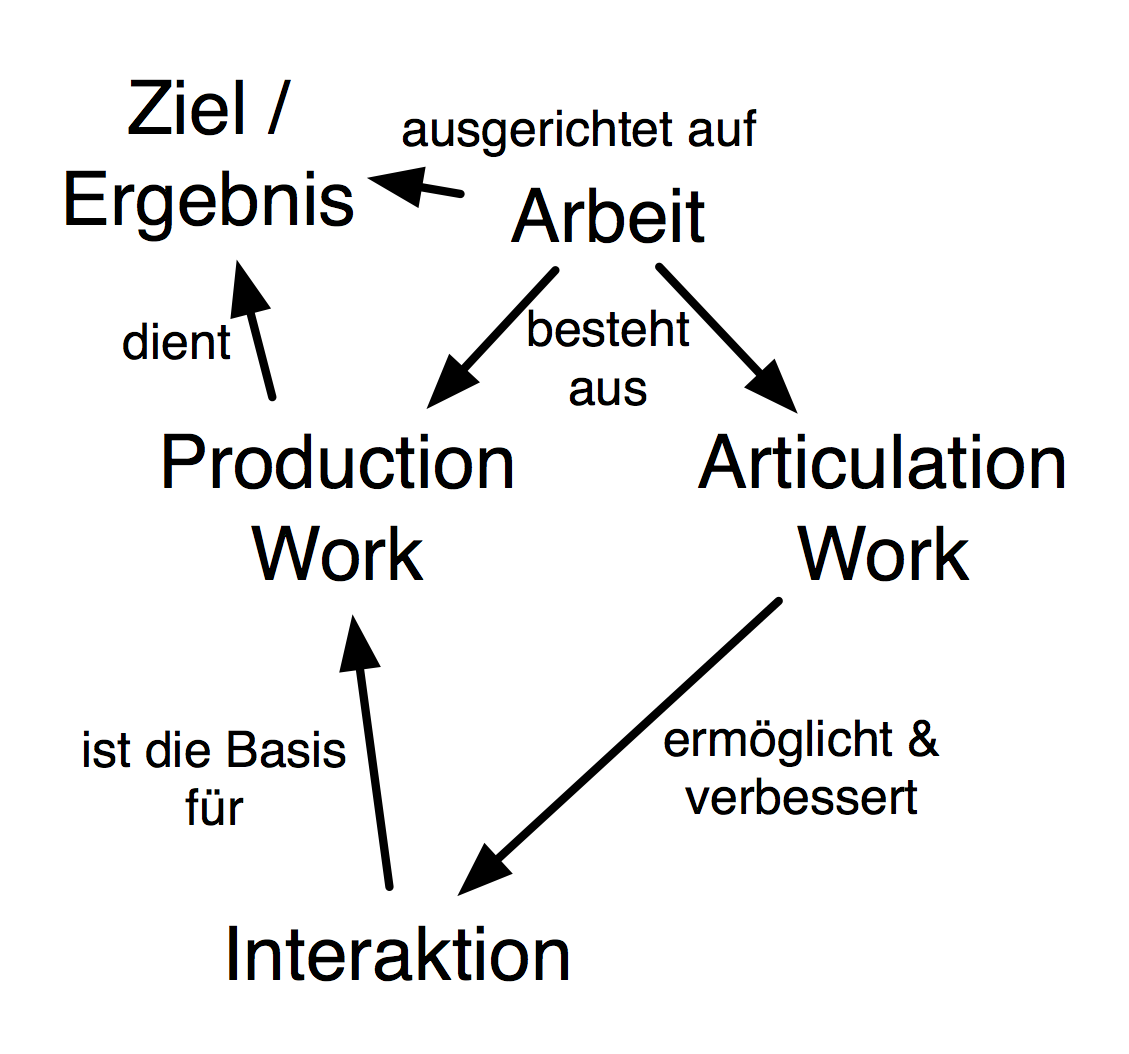
\includegraphics[height=3in]{img/ArticulationWork/ArbeitInteraktion.png}
	\caption{Struktur von Arbeitsabläufen}
	\label{fig:img_ArticulationWork_ArbeitInteraktion}
\end{figure}

Teile eines Arbeitsablaufs dienen also der Zielerreichung an sich („Production Work“). Andere Teile dienen der Abstimmung zwischen den involvierten Akteuren, um ein gemeinsames Verständnis über die jeweiligen Schnittstellen – also die Berührungspunkte zwischen den Tätigkeiten – zu entwickeln. Diese „Koordination“ ist kritisch für den Erfolg von kooperativer Arbeit \citep{Strauss93} und wird als „Articulation Work“ bezeichnet.\footnote{\emph{„Without an understanding of articulation, the gap between requirements and the actual work process in the office will remain inaccessible to analysis. That is, it will be possible to describe tasks in an idealized form but not to describe actual situations.“}\citep{Gerson86}} „Articulation Work“ ist damit ein Enabler für funktionierende Kommunikation und Koordination im eigentlichen Arbeitsprozess\footnote{\emph{"Reconciling incommensurate assumptions and procedures in the absence of enforceable standards is the essence of articulation. Articulation consists of all the tasks involved in assembling, scheduling, monitoring, and coordinating all of the steps necessary to complete a production task."}\citep{Gerson86}}. 

\begin{figure}[htbp]
	\centering
		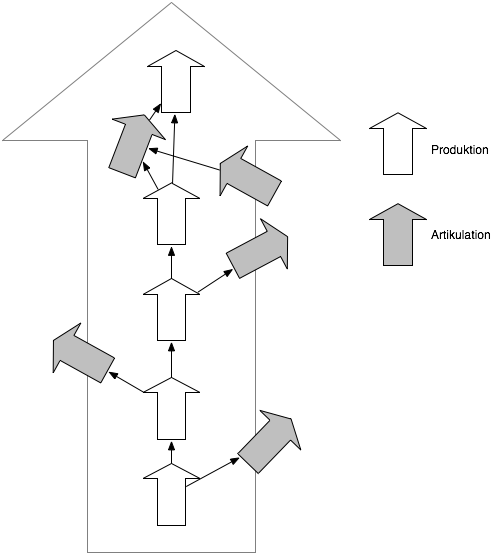
\includegraphics[height=3in]{img/ArticulationWork/ArtikulationProduktion.png}
	\caption{Konzeptualisierung von „Arbeit“ nach \citep{Strauss85} und \citep{Fujimura87}}
	\label{fig:img_ArticulationWork_ArtikulationProduktion}
\end{figure}

Der Begriff „Articulation Work“ ist im Englischen zweideutig und von Strauss bewusst so gewählt. Einerseits wird damit ausgedrückt, dass \emph{Arbeit} ("Work") artikuliert wird, andererseits zeigt der Begriff, das die \emph{Artikulation} selbst ebenfalls Arbeit ist (also Zeit und Ressourcen in Anspruch nimmt) und auch also solche wertgeschätzt werden muss \citep{Fujimura87}. „Articulation Work“ ist kein klar abgegrenztes und strukturiertes Konzept – sie tritt je nach Arbeitssituation in unterschiedlichen Spielarten auf. Die Unterscheidung dieser Arten von „Articulation Work“ ist für die Unterstützung derselben relevant und wird daher im folgenden Abschnitt genauer betrachtet.
% section begriffsbestimmung (end)

\section{Kontext} % (fold)
\label{sec:kontext}
Arc of Work, Due Process, ...
% section kontext (end)

\section{Arten von Articulation Work} % (fold)
\label{sec:arten_von_articulation_work}

Strauss argumentiert, dass Artikulation immer passieren muss (und passiert), wo Menschen zusammenarbeiten, um zu vermeiden, dass unbekannte Aspekte Probleme bei der Durchführung der Arbeit verursachen \citep{Strauss88}. „Articulation Work“ ist kein revolutionäres Konzept, sondern fasst Tätigkeiten unter einem Begriff zusammen, die seit jeher Teil jeder Zusammenarbeit zwischen Menschen sind. Grundsätzlich geht Strauss davon aus, dass Artikulation immer abläuft, egal wie einfach oder kompliziert, wie eingespielt oder neuartig eine (Zusammen-)Arbeit ist \citep{Strauss88}. Sehr wohl existieren jedoch Unterschiede in der Qualität der Arbeit, die sich auf die Form der Artikulation auswirken, die zu deren Abstimmung notwendig ist: \emph{„A useful fundamental distinction between classes of interaction is between the routine and the problematic. Problematic interactions involve 'thought', or when more than one interactant is involved then also 'discussion'.“} \citep{Strauss93}. Dieses Zitat zeigt im Übrigen auch, dass „Interaction“ im Sinne von Strauss nicht unbedingt ein kollektives Phänomen ist, sondern auch individuell (im Bezug auf die (unbelebte) Umgebung) auftreten kann.

Je komplexer („problematic“) eine Interaktion ist, desto notwendiger wird laut Strauss eine explizite Beschäftigung mit dem Vorgang der Artikulation. Bei einfachen, eingespielten („routine“) Interaktionen bleibt die Artikulation zumeist implizit, verborgen und informell \citep{Hampson05} (entsprechend der „Sozialisation“ in Nonaka \& Takeuchis SECI-Zyklus \citep{Nonaka95}). Ein grundlegendes Problem, dass Artikulation für jeden noch so einfach erscheinend Arbeitsvorgang potentiell relevant macht, spricht Strauss mit den Worten von Hughes unmittelbar nach der Definition von „problematic interaction“ an: \emph{„[O]ne man's routine of work is made up of the emergencies of other people“} \citep{Hughes71} zitiert nach \citep{Strauss93}.

„Articulation Work“ tritt also in zwei Qualitäten auf. Ist der Bedarf zur Abstimmung bekannt und werden Tätigkeiten zur Abdeckung dieses Bedarf bewusst durchgeführt, so spricht man von \emph{expliziter} „Articulation Work“ \citep{Strauss88}\citep{Fjuk97}. Die Abstimmung von Tätigkeiten, die ständig während der Zusammenarbeit unbewusst ausgeführt wird, bezeichnet man als implizite „Articulation Work“. Letztgenannte Art ist es auch, die von den Arbeitenden „automatisch“ zur Anwendung gebracht wird, sobald Änderungen in der Arbeitsumgebung oder Probleme auftreten \citep{Strauss88}. Implizite „Articulation Work“ stößt aber an ihre Grenzen, wenn die Arbeitssituation als „problematisch“ \citep{Strauss88} oder „komplex“ \citep[][S. 23f]{Schmidt90} wahrgenommen wird. Es wird dann notwendig, dezidierte Abstimmungs-Aktivitäten anzustoßen, also explizite „Articulation Work“ durchzuführen.
% section arten_von_articulation_work (end)

\section{Systematisierung von Articulation Work} % (fold)
\label{sec:systematisierung_articulation_work}

Fjuk (Vergleich mit Activity Theory)
Hampson (Vergleich mit Wissensspirale?)

Neben der Unterscheidung zwischen impliziter und explizter Articulation Work anhand der Komplexität der zugrundeliegenden Interaktion führt Strauss keine systematische Betrachtung von Articulation Work hinsichtlich deren Ausprägungen durch. Offensichtlich wird in seinen Text jedoch, dass es Articulation Work als einzigartiges, beobachtbares und eindeutig also solche indentifizierbares Phänomen nicht gibt. Abhängig vom betrachteten Arbeitsablauf, der Arbeitsumgebung und den beteiligten Personen zeigt sich Articulation Work in unterschiedlichen Formen. Um eine strukturierte, differenzierte Betrachtung zu ermöglichen und in der Folge Unterstützungsmaßnahmen ableiten zu können, ist eine Einführung einer Systematik sinnvoll.

In der Literatur existieren zwei Ansätze zur Differenzierung zwischen unterschiedlichen Arten von Articulation Work. Fjuk (REF) stellen Articulation Work der Activity Theory (REF) gegenüber und unterscheiden so verschiedene Ebenen. Hampson (REF) führen ein Raster ein, das Articulation Work hinsichtlich der Art des Arbeitsprozesses unterschiedet, in dem sie zur Anwendung kommt. Beide Ansätze werden in der Folge im Detail beschrieben und bezüglich ihrer Implikationen für diese Arbeit betrachtet.

\subsection{Systematik nach Fjuk, Smørdal und Nurminen}
\label{sub:systematik_fjuk}

\citet{Fjuk97} betrachten Articulation Work im Kontext von \gls{CSCW} und versuchen ein konzeptuelles Framework zu entwickeln, das die Rolle von Computersystemen im Kontext indvidueller und kollektiver Tätigkeiten erklärt -- sie entwickeln also ein Erklärungsmodell für die Funktionsweise sozio-technischer Systeme (REF). Ansatzpunkt ist dabei die Betrachtung von Computersystemen als Arbeitsgegenstände. Arbeitsgegenstände als solche werden von Strauss jedoch nicht explizit in seinen Ausführungen berücksichtigt, so dass sich hier eine konzeptuelle Lücke ergibt. Diese versuchen die Autoren mit der Einführung der Activity Theory (REF) zu schließen.  

\subsection{Systematik nach Hampson und Junor}
\label{sub:systematik_hampson}
% section systematisierung_articulation_work (end)

\section{Unterstützung von Articulation Work} % (fold)
\label{sec:unterstützung_von_articulation_work}

Nach den ersten Arbeiten von Strauss zum Thema „Articulation Work“ wurde das Konzept rasch als Erklärungsmodell für die Vorgänge im Zuge kooperativer Arbeit aufgenommen und darauf basierend Maßnahmen zur Unterstützung derselben abgeleitet. Anhand der historischen Entwicklung von Mitte der 1980er-Jahre bis Ende des ersten Jahrzehntes des neuen Jahrtausends werden im Folgenden diese Maßnahmen beschrieben, in den jeweiligen Anwendungskontext gesetzt und auch hinsichtlich des zu unterstützenden Verständnisses von „Articulation Work“ betrachtet. Hierbei werden alle Arbeiten berücksichtigt, die sich direkt auf den von Strauss geprägten „Articulation Work“-Begriff beziehen.

Zur strukturierten Umsetzung der Betrachtung der historischen Entwicklung von „Articulation Work“ wird ein einheitlicher Raster angewandt, anhand dessen die aus unterschiedlichen Forschungsgebieten stammenden und in unterschiedlichen Anwendungsdomänen angewandten Arbeiten einander gegenüber gestellt werden können. Neben den eigentlichen Unterstützungsmaßnahmen ist zur Bewertung derselben auch Kontextinformation notwendig, die die unterschiedlichen Ansätze offenlegt. Folgende Merkmale einer Arbeit werden dazu betrachtet:
\begin{description}
 \item[Forschungsdomäne] Forschungsgebiet aus dem das Konstrukt "Articulation Work" betrachtet wird bzw. in dessen Kontext es zur Anwendung gebracht wird.
 \item[Untersuchungsdomäne] Abstraktes oder konkretes Problemfeld, in dem "Articulation Work" als Anaylsedimension oder zur Ableitung von Maßnahmen angewandt wird.
 \item[Verständnis von Articulation Work] Bei der Betrachtung der Untersuchungsdomäne zur Anwendung gebrachte Definition von "Articulation Work" (ggf. auch in Abgrenzung zu anderen Arten von Arbeit).
 \item[Auftretende Phänomene] Tätigkeiten und/oder Handlungsweisen, die im Zuge von "Articulation Work" auftreten und ggf. unterstützt werden können
 \item[Unterstützung] Konkrete oder abstrakte Maßnahmen oder Werkzeuge, die zur Unterstützung von "Articulation Work" vorgeschlagen und/oder umgesetzt werden.
 \item[Auftretende Effekte] Tatsächliche oder vermutete Auswirkungen der Unterstützung auf die durchgeführte "Articulation Work"
\end{description}

Die als relevant betrachteten Publikationen sind methodisch höchst unterschiedlich ausgerichtet. Ein großer Anteil beschreibt rein empirisch-deskriptiv ein beobachtetes Phänomen und zieht Schlüsse hinsichtlich möglicher bzw. notwendiger Ausprägungen von "Articulation Work" in bestimmten Anwendungsdomänen. Ein anderer Teil fokussiert auf die organisationale und/oder technische Unterstützung von "Articulation Work", zum Teil ohne auf eigene empirische Ergebnisse aufzubauen oder diese zu erheben. Aus diesem Grund kann das oben angegebene Raster nicht immer vollständig befüllt werden. Wo hinsichtlich einer bestimmten Dimension keine Information vorhanden ist, wird explizit im Text darauf hingewiesen. Wo mehrere Publikation eines Autors oder einer Gruppe zum gleichen Forschungsgegenstand existieren, wurden diese in einem Abschnitt zusammengefasst und in der jeweiligen Einleitung auf die der Beschreibung zugrundeliegenden Publikationen verwiesen.

%TEMPLATE
\subsection{Papertitel / Titel des Forschungsprojekts}

Angabe der zugrundeliegenden Publikation sowie einer kurzen Zusammenfassung des Inhalts

\paragraph{Forschungsdomäne}

\paragraph{Untersuchungsdomäne}

\paragraph{Verständnis von Articulation Work}

\paragraph{Auftretende Phänomene}

\paragraph{Unterstützung}

\paragraph{Auftretende Effekte}
%TEMPLATE

\subsection{Work and the Division of Labor}

In dieser Publikation \citep{Strauss85} beschreibt Strauss zum ersten Mal sein Konzept „Articulation Work“. Er motiviert seine Forschung mit Erklärungs-Lücken, die in der Konzeptualisierung von kooperativer Arbeit bzw. Arbeitsteilung bestehen. Ziel ist es, mit den entwickelten Ansätzen nicht nur Arbeit(steilung) erklären zu können sondern auch weitergehende Forschung zu ermöglichen bzw. dieser als Leitprinzipen zugrunde zu liegen. 

\paragraph{Forschungsdomäne}
Strauss' Hintergrund, auf Basis dessen die hier betrachtete Publikation geschrieben wurde, ist die Soziologie (im konkreten Artikel die Medizinsoziologie \citep[vgl.][]{Siegrist05}). Methodisch wendet er den von ihm mitgeprägten „Grounded Theory“-Ansatz \citep{Glaser77} an, mithilfe dessen aus Feldbeobachtungen und deren systematischer, qualitativer Auswertung Theorien abzuleiten, die das Verhalten und die Interaktion der beobachteten Akteure erklärt.

\paragraph{Untersuchungsdomäne}
Neben einer konzeptuellen Erörterung der kooperativen Arbeit zugrunde liegenden Denkmodelle und Betrachtungsmuster (siehe Abschnitt \ref{sec:kontext}) werden  

\paragraph{Verständnis von Articulation Work}

\paragraph{Auftretende Phänomene}

\paragraph{Unterstützung}

\paragraph{Auftretende Effekte}
%TEMPLATE

\subsection{Gegenüberstellung und Zusammenfassung} % (fold)
\label{sub:gegenüberstellung_und_zusammenfassung}

% subsection gegenüberstellung_und_zusammenfassung

% section unterstützung_von_articulation_work (end)

\section{Fazit} % (fold)
\label{sec:fazit}

\textbf{hier muss eine zusammenfassende Tabelle der in der Literatur verfügbaren Information rein}

Die Zielsetzung von „Articulation Work“ formulieren die Proponenten des Ansatzes - allen voran Strauss - klar aus. Offen bleiben jedoch bei allen Autoren direkten Aussagen zum eigentlichen Gegenstand von „Articulation Work“ – also Allem was von den beteiligten Individuen zu artikulieren ist – und den notwendigen Leistungen der Individuen im Prozess der Artikulation. Aussagen zu diesen Aspekten sind aber für die Entwicklung von Ansätzen zur Unterstützung von expliziter „Articulation Work“ notwendig. 

Strauss ist sich dieser Auslassung bewusst\footnote{\emph{„[\ldots] many social scientist pay almost no attention to interior activity: ignoring it, taking it for granted, but leaving it unexamined, or giving it the kind of abstract but not very detailed analysis [\ldots]“}\citep[][S. 131]{Strauss93}}, und beschäftigt sich in späteren Arbeiten \citep{Strauss93} auch mit jenen kognitiven Vorgängen, die von ihm als „thought processes“ oder „mental activities“ bezeichnet werden und die untrennbar mit jeder Art von Tätigkeit und Interaktion verbunden sind\footnote{\emph{„These [thought processes] accompany visible action, as well as precede and follow in conditional and consequential modes“}\citep[][S. 146]{Strauss93}} und diese beeinflussen\footnote{\emph{„Even well-grooved, routine action and interaction may be accompanied by thought [\ldots] directly relevant to the work at hand. As I vacuum the house, barely noticing my movements, still I give myself commands [\ldots]“}\citep[][S. 132]{Strauss93}}. 

Im Kontext der Abstimmung von Tätigkeiten kommt den „thought processes“ der Individuen große Bedeutung zu, da sie den sichtbaren individuellen Handlungen zugrunde liegen bzw. diese beeinflussen. „Articulation Work“ wirkt sich also auf die „thought processes“ der beteiligten Individuen aus. „Thought processes“ umfassen \emph{„images, imaginations, projections of scenes, [...] flashes of insight, rehearsals of action, construction and reconstruction of scenarios, the spurting up of metaphors or comparisons, the reworking and reevaluating of past scenes and one's actions within them, and so on and on“} \citep[][S. 130]{Strauss93} - also im Wesentlichen alle kognitiven Vorgänge, die unmittelbar oder mittelbar im Zusammenhang mit den sichtbaren Arbeitsaspekten, insbesondere den Tätigkeiten zur Zielerreichung und der wahrgenommenen Arbeitsumgebung, stehen. Strauss interessiert sich allerdings ausschließlich für die dynamischen Aspekte der Interaktion zwischen Individuen, nicht aber für die Ausgangspunkte und Ergebnisse der zugrunde liegenden „thought processes“.\footnote{\emph{„I use the gerund 'ing' after 'symbol' [bei der Beschreibung von 'symbolizing', Anm.] to signify that my principal interest is, again, in interaction rather than its products, for symbols are precipitates of interaction“}\citep[][S. 149]{Strauss93}}  Wie bereits oben erwähnt sind aber die Repräsentationen, auf den „thought processes“ beruhen und operieren, für die Unterstützung von „Articulation Work“ von Interesse. Die kognitions-wissenschaftlichen Ansätze zu Schemata (\citep{Rumelhart78} \citep[vgl. nach ][]{Hanke06}) und mentalen Modellen (\citep[vgl. ]{Seel91}) sind ein Erklärungsansatz für diese Lücke.

% section fazit (end)
% chapter articulation_work (end)


\part{Evaluierung} % (fold)
\label{prt:evaluierung}

\chapter{Untersuchungsdesign} % (fold)
\label{cha:untersuchungsdesign}

Die Evaluierung des in der vorliegenden Arbeit beschriebenen Werkzeuges wurde entsprechend der in Kapitel \textbf{XY} vorgestellten konzeptuellen Zusammenhänge mit Fokus auf unterschiedliche Gesichtspunkte durchgeführt. Die beiden grundlegenden Untersuchungsfragen sind
\begin{itemize}
	\item Unterstützen Werkzeug und Methode Articulation Work?
	\item Ermöglichen und unterstützen die Teilwerkzeuge des Modellierungstisches Articulation Work?
\end{itemize}
Die erste Frage setzt im oberen Bereich der Argumentationskette an (\textbf{Bild einfügen}) und untersucht, ob Articulation Work bei Einsatz des Werkzeugs tatsächlich auftritt bzw. ob diese unterstützt wird. Die zweite Frage geht wiederum von der Unterstützung von Articulation Work aus, betrachtet hierbei jedoch den Beitrag der vorhandenen Teilwerkzeuge und zielt auf die Untersuchung der Übereinstimmung zwischen intendierter (bzw. aus den Anforderungen ableitbaren) und tatsächlicher Einsatzgebiete ab. Die diesen Fragen zugrunde liegenden Annahmen und die jeweiligen Ansätze zur Messung werden in den nächsten beiden Abschnitten behandelt. Der letzte Abschnitt dieses Kapitels beschreibt dann die konkrete Planung der Untersuchung und die im Einzelnen durchgeführten Untersuchungs-Phasen. 

\section{Frage 1 – Unterstützung von Articulation Work} % (fold)
\label{sec:frage_1_unterstützung_von_articulation_work}

Axiom 1:
Erfolgreiche Articulation Work zeigt sich an der Production Work (-> Ref. Strauss)

Axiom 1,5:
Erfolgreiche Production Work zeigt sich an der Zielerreichung (-> Erfolg) (-> Ref. Fujimura)

Axiom 2: 
(Geschäfts-)Erfolg steht in direktem Zusammenhang mit funktionierender Interaktion (-> Ref. 

Messung:
Die Unterstützung der Articulation Work kann an Ihren Auswirkungen auf die Production Work gemessen werden, dort im speziellen an der Qualität der Interaktion ("Work rests ultimately on Interaction"). Messpunkte können dabei die Akteure oder die Ergebnisse der kollaborativen Arbeit sein.

Misst man an den Akteuren, so kann die subjektive Zufriedenheit mit dem Arbeitsprozess (Verlauf der Interaktion) und/oder das beobachtbare Verhalten der Akteure als Merkmal herangezogen werden. Ersteres kann methodisch durch qualitative Interviews (ggf. unterstützt durch Modelle -> Herrmann, Jahnke 2008) beurteilt werden. Zweiteres kann durch Techniken der Interaktionsanalyse bewertet werden, wobei insbesondere die Gegenüberstellung der tatsächlichen zu den vereinbarten Interaktionsmodalitäten und die Veränderung dieser Vereinbarung über die Zeit von Interesse ist. Dazu ist eine Externalisierung der Vereinbarungen zu unterschiedlichen Zeitpunkten notwendig. 

Misst man an den Ergebnissen der kollaborativen Arbeit, so kann die subjektive Zufriedenheit mit dem Ergebnis und die "verobjektivierte" (Experten)-Beurteilung der Qualität des Ergebnisses als Merkmal verwendet werden. Ersters wird wiederum qualitativ in Befragungen zu erheben sein. Die Qualität des Ergebnisses wird von Experten an noch zu definierenden Merkmalen gemessen werden, an denen sich die Interaktion bei der Erstellung zeigt (etwa: Stilbrüche, etc.). Bei der Beurteilung der Qualität der Ergebnisse ist vor allem die Gegenüberstellung zu Ergebnissen von Interesse, die ohne Unterstützung der Articulation Work entstanden sind. Dementsprechend kann der Einsatz einer Kontrollgruppe sinnvoll sein.

\section{Frage 2 – Beitrag und Verwendung der Teilwerkzeuge} % (fold)
\label{sec:frage_2_beitrag_und_verwendung_der_teilwerkzeuge}

Axiom: Articulation Work kann durch Strukturlegetechniken unterstützt werden

Messung:
Die Verwendung der einzelnen Werkzeuge kann durch Beobachtung und Befragung modellierender Personen sowie der Untersuchung der Modellierungsergebnisse beurteilt werden. Messpunkte sind damit wiederum die Akture und die Ergebnisse der Artikulation. Bei der Messung ist in diesem Zusammenhang kein kollaboratives Setting notwendig, da nicht die Auswirkungen des Werkzeugs auf Interaktion sondern die Verwendung des Werkzeugs selbst untersucht werden soll. Die Modellierung wird also von einzelnen Personen durchgeführt (Selbst-Artikulation, Externalisierung eignere mentaler Modelle). Durch Auswertung der Modellierungen aus Evaluierung I lässt sich ein etwaiger Unterschied in der Verwendung der Werkzeuge bei kollaborativen Settings belegen.

% section frage_2_beitrag_und_verwendung_der_teilwerkzeuge (end)
% section frage_1_unterstützung_von_articulation_work (end)

\section{Untersuchungsablauf} % (fold)
\label{sec:untersuchungsablauf}

Die Evaluierung selbst wurde in drei Phasen gegliedert, deren Untersuchungsfokus auf 
\begin{itemize}
	\item der Verwendbarkeit des Werkzeugs an sich,  
	\item dessen Eignung zur Unterstützung von "Articulation Work" in Lehr- und Lern-Szenarien und
	\item dessen Eignung zur Unterstützung von "Articulation Work" beim Einsatz in Unternehmen
\end{itemize}
lag. Die erste Phase ist als Vorlauf zu sehen, der nicht unmittelbar der Beantwortung der Untersuchungsfragen diente, sondern auf die rein explorative Untersuchung der tatsächlichen Verwendbarkeit des Werkzeuges (im Sinne der Verständlichkeit und Robustheit) abzielte. Die beiden folgenden Phasen decken die Bearbeitung der eigentlichen Untersuchungsfragen ab, wobei durch den unterschiedlichen Einsatzkontext versucht wurde die verschiedenen Anwendungsgebiete des Werkzeugs in die Untersuchung einfließen zu lassen.

Im Zuge der Evaluierungen wurde das Werkzeug unter realen Einsatzbedingungen getestet. Unter "real" ist hier zu verstehen, dass die testenden Benutzer mit der Bedienung des Werkzeugs vorab nicht vertraut waren und dass die Aufgabenstellung stets einen konkreten Bezug zu einem für die jeweiligen Personen relevanten Arbeitsszenario aufwies. In den folgenden Abschnitten wird im Detail auf die Konzeption der einzelnen Phasen und den jeweiligen Beitrag zur Beantwortung der Untersuchungsfragen eingegangen.

\subsection{Phase 1 – Verwendbarkeit} % (fold)
\label{sub:phase_1_verwendbarkeit}

% subsection phase_1_verwendbarkeit (end)

\subsection{Phase 2 – Lehr- und Lern-Szenarien} % (fold)
\label{sub:phase_2_lehr_und_lern_szenarien}


% subsection phase_2_lehr_und_lern_szenarien (end)

\subsection{Phase 3 – Unternehmenseinsatz} % (fold)
\label{sub:phase_3_unternehmenseinsatz}

% subsection phase_3_unternehmenseinsatz (end)
% section untersuchungsablauf (end)

% chapter untersuchungsdesign (end)

\chapter{Untersuchungsergebnisse} % (fold)
\label{cha:untersuchungsergebnisse}

\section{Erhobene Daten} % (fold)
\label{sec:erhobene_daten}

\subsection{Phase 1} % (fold)
\label{sub:phase_1}

In Phase 1 wurden 9 Modellierungsdurchgänge mit insgesamt 18 Personen durchgeführt. An dem vorangegangenen Pretest nahmen 12 Personen teil.
% subsection phase_1 (end)

\subsection{Phase 2} % (fold)
\label{sub:phase_2}

In Phase 2 wurden Untersuchungen im Rahmen zweier Lehrveranstaltungen durchgeführt. An der ersten Untersuchung nahmen 18 Studierende der Wirtschaftsinformatik teil, die in Gruppen zu 2 Personen insgesamt 17 Modellierungsdurchgänge durchführten. An der zweiten Untersuchung nahmen 54 Studierende in Gruppen zu 3 Personen an insgesamt 18 Modellierungsdurchgängen teil.
% subsection phase_2 (end)

\subsection{Phase 3} % (fold)
\label{sub:phase_3}

% subsection phase_3 (end)
% section erhobene_daten (end)

\section{Auswertung \& Interpretation} % (fold)
\label{sec:auswertung_&_interpretation}

% section auswertung_&_interpretation (end)
% chapter untersuchungsergebnisse (end)
% part evaluierung (end)


\bibliography{/Users/oppl/Documents/Dokumente/Literatur/archiv}

\addcontentsline{toc}{part}{Index}
\printindex

\appendix
%\include{Anhang}

\end{document}